%----------------------------------------------------------------------------------------
%    PACKAGES AND THEMES
%----------------------------------------------------------------------------------------
\documentclass[aspectratio=169,xcolor=dvipsnames]{beamer}
\makeatletter
\def\input@path{{theme/}}
\makeatother
\usetheme{CleanEasy}
\usepackage[utf8]{inputenc}
\usepackage{lmodern}
\usepackage[T1]{fontenc}
% \usepackage[brazil]{babel}
\usepackage{fix-cm}
\usepackage{amsmath}
\usepackage{mathtools}
\usepackage{physics}
\usepackage{listings}
\usepackage{xcolor}
\usepackage[dvipsnames]{xcolor}
\usepackage{hyperref}
\usepackage{changepage}
\usepackage{graphicx} % Allows including images
\usepackage{booktabs} % Allows the use of \toprule, \midrule and \bottomrule in tables
\usepackage{tikz}
\usetikzlibrary{positioning, shapes, arrows, calc, decorations.pathreplacing, arrows.meta, backgrounds, patterns, overlay-beamer-styles}
\usepackage{etoolbox}
\usepackage{animate}
\usepackage{appendixnumberbeamer}

\usepackage[makeroom]{cancel}

\usepackage{xpatch}
\xpatchcmd{\boxed}{%
\fbox}{%
\fcolorbox{red}{white}}{}{}

\newcommand{\myarrow}[1][]{
  \begin{tikzpicture}[#1]
  \draw[-{Latex[length=2mm, width=2mm]}, draw=black]
    (0,0.5em) -- (0,0) -- ++(1em,0);
  \end{tikzpicture}
}

\newcommand\boldblue[1]{\textcolor{blue}{\textbf{#1}}}
\newcommand\boldred[1]{\textcolor{red}{\textbf{#1}}}

% Adjustable gray percentage when hiding text
\newcommand{\graylevel}{90} % 0 = no gray, 100 = fully gray

\definecolor{verylightgray}{gray}{0.9}

\newcommand{\textcolorg}[2]{%
  \textcolor{verylightgray!\graylevel!#1}{#2}%
}

\newcommand\credit[2]{
        \\ \vspace{-0.5em}
        {\color{gray}\scriptsize
        \hfill
        #1
        \hspace{#2}}
        }
        
\definecolor{mylightgray}{gray}{0.96}

\newcommand\mytitle[1]{\textcolor{OliveGreen}{#1}}

%----------------------------------------------------------------------------------------
%    LAYOUT CONFIGURATION
%----------------------------------------------------------------------------------------



% Configure code listings
\lstset{
  basicstyle=\ttfamily\small,
  keywordstyle=\color{blue},
  commentstyle=\color{green!60!black},
  stringstyle=\color{red},
  showstringspaces=false,
  breaklines=true,
  frame=single,
  rulecolor=\color{black!30},
  backgroundcolor=\color{black!5},
  numbers=left,
  numberstyle=\tiny\color{black!70},
  numbersep=5pt
}

%----------------------------------------------------------------------------------------
%    TITLE PAGE
%----------------------------------------------------------------------------------------


%---------------------------------------------


\title[Navier Stokes equations]{Approximations of the Navier Stokes equations in ocean, atmosphere and ice-sheet modeling}

%\subtitle[Trial Lecture for Master's Course]

\author[A. Robinson]{Alexander Robinson }  % \inst{1}

%\institute[AWI]{\inst{1}%
%  Faculty of Physics\\
%  Alfred Wegener Institute, Helmholtz Centre for Polar and Marine Research
%  \and
%  \inst{2}%
%  Faculty of Chemistry\\
%  Very Famous University 
%}


\vspace{-2cm}\date{11. July 2025}
% Define positions for logos on title page
% \titlegraphic{
%   \begin{tikzpicture}[remember picture, overlay]
%     % 
%     \node[anchor=south west, xshift=0.5cm, yshift=0cm] at (current page.south west) {
%       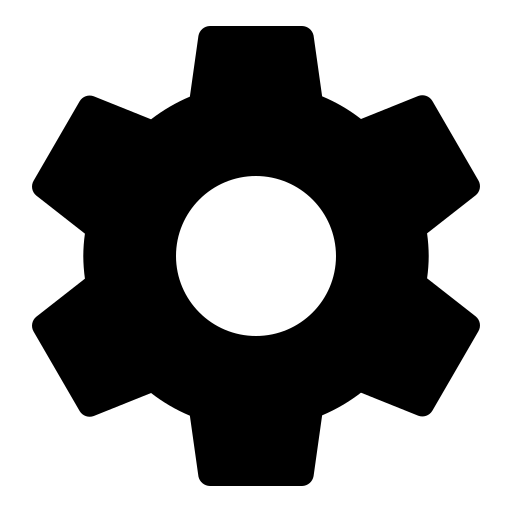
\includegraphics[height=1.3cm]{logos/CleanEasy-logo1.png}
%     };

%     % 
%     \node[anchor=south west, xshift=2.5cm, yshift=0cm] at (current page.south west) {
%       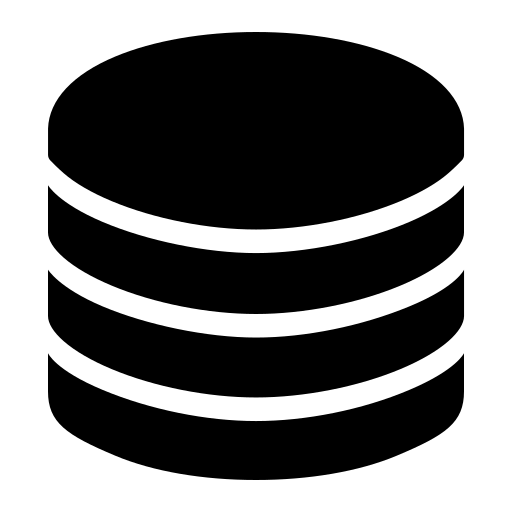
\includegraphics[height=0.9cm]{logos/CleanEasy-logo2.png}
%     };
    
%     % 
%     \node[anchor=north east, xshift=-0.8cm, yshift=-0.3cm] at (current page.north east) {
%       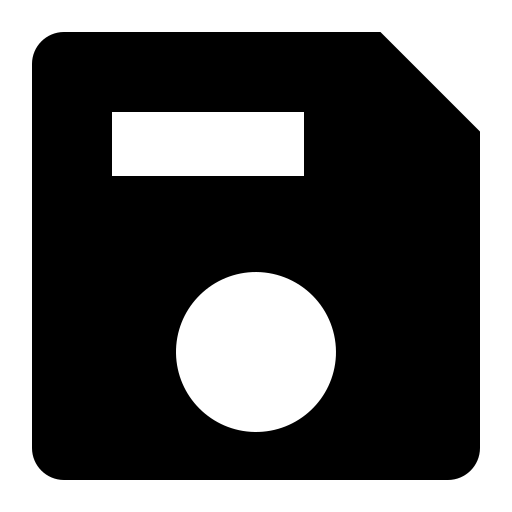
\includegraphics[height=1.1cm]{logos/CleanEasy-logo3.png}
%     };
    
%     %
%     \node[anchor=north east, xshift=-2.8cm, yshift=-0.3cm] at (current page.north east) {
%       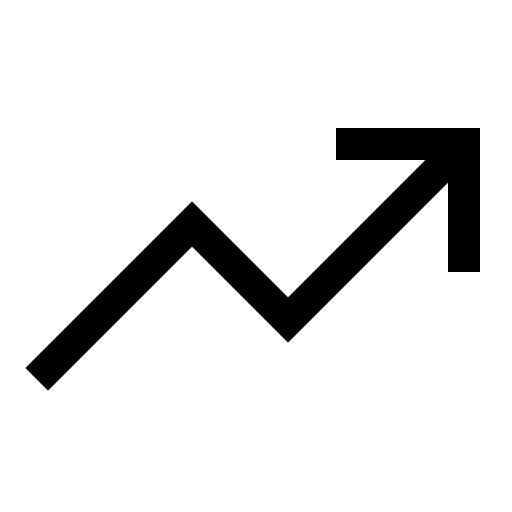
\includegraphics[height=1.4cm]{logos/CleanEasy-logo4.png}
%     };
%   \end{tikzpicture}
% }


%----------------------------------------------------------------------------------------


\begin{document}

\begin{frame}[plain]
  \titlepage
\end{frame}

%\begin{frame}[plain]{Contents}
%  \tableofcontents
%\end{frame}

\begin{frame}{Motivation}

    \begin{columns}
        \begin{column}{0.02\textwidth}
        \end{column}
        \begin{column}{0.5\textwidth}
          
          \vspace{0.3cm}
          
          Many Earth-system components are essentially dynamic fluids governed by an \emph{equation of state} combined with the laws of 
          
          \vspace{0.3cm}
          
          \begin{itemize}
              \item Conservation of momentum 
              \item Conservation of mass 
              \item Conservation of energy
          \end{itemize}
          
          \vspace{0.3cm}

          Modeling these systems helps us to understand them and to make predictions.
        \end{column}
          
        \begin{column}{0.48\textwidth}
            \centering
            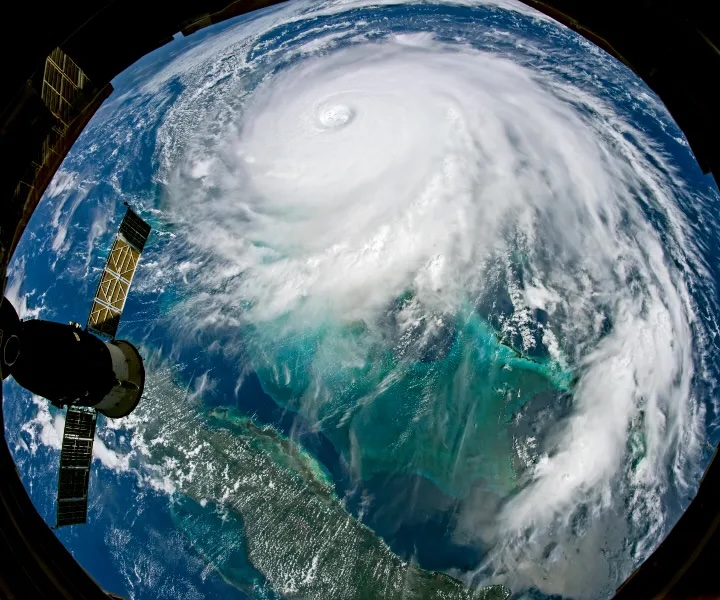
\includegraphics[width=0.9\textwidth]{figs/Fig-nasa-dorian.jpg}
            \credit{NASA - Hurricane Dorian}{5pt}
        \end{column}
    \end{columns}
    
\end{frame}

\begin{frame}[t]{Motivation}

    \hspace{2em}The \textbf{momentum balance} of all of these systems \\ 
    \hspace{2em}can be described by the 
    \textbf{Navier-Stokes equations}. 

    \begin{columns}
        \begin{column}{0.32\textwidth}
            \centering
            \hspace{2em}\textbf{Atmosphere}
            \vspace{0.2cm} \newline
            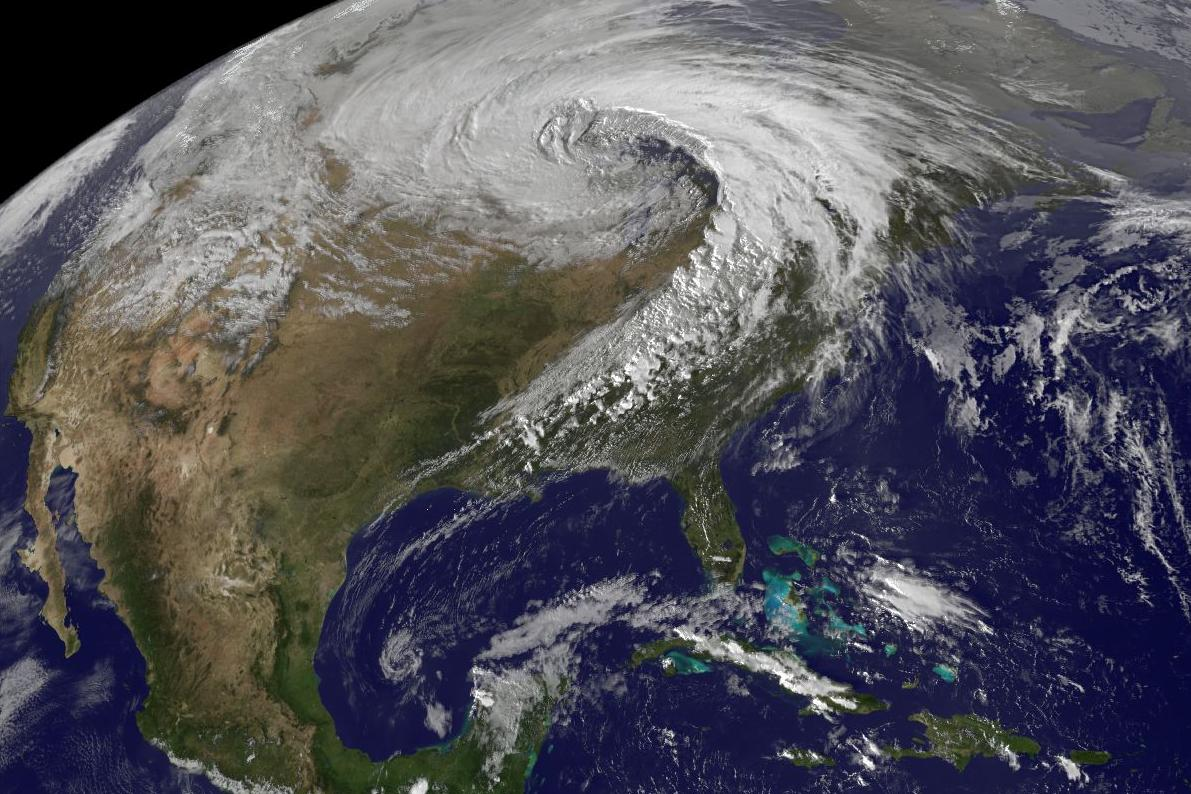
\includegraphics[width=0.9\textwidth]{figs/Fig-MidLatCyclone_2010-10-26_low_pressure.jpg}
            \credit{NOAA}{5pt}
        \end{column}
        \begin{column}{0.36\textwidth}
            \centering
            \hspace{2em}\textbf{Ocean}
            \vspace{0.2cm} \newline
            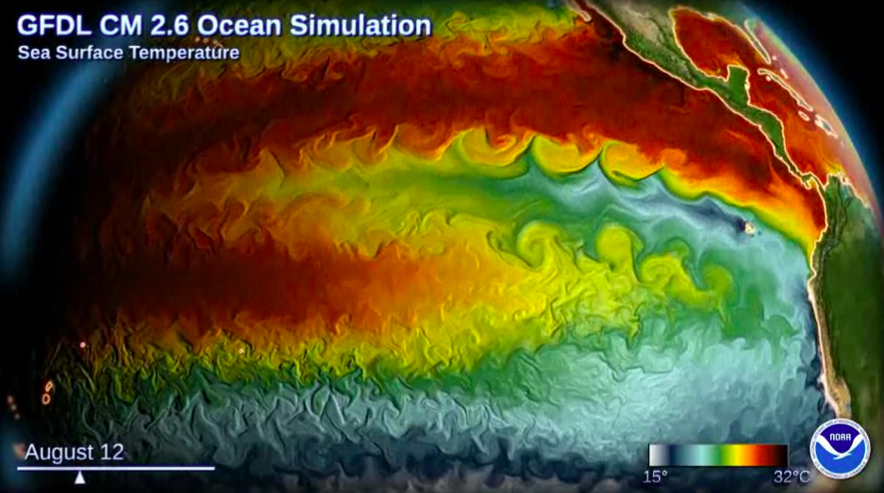
\includegraphics[width=0.9\textwidth]{figs/Fig-cm2.6-mesoscale-eddies.png}
            \credit{NOAA}{3pt}
        \end{column}
        \begin{column}{0.32\textwidth}
            \centering
            \hspace{2em}\textbf{Ice sheets}
            \vspace{0.2cm} \newline
            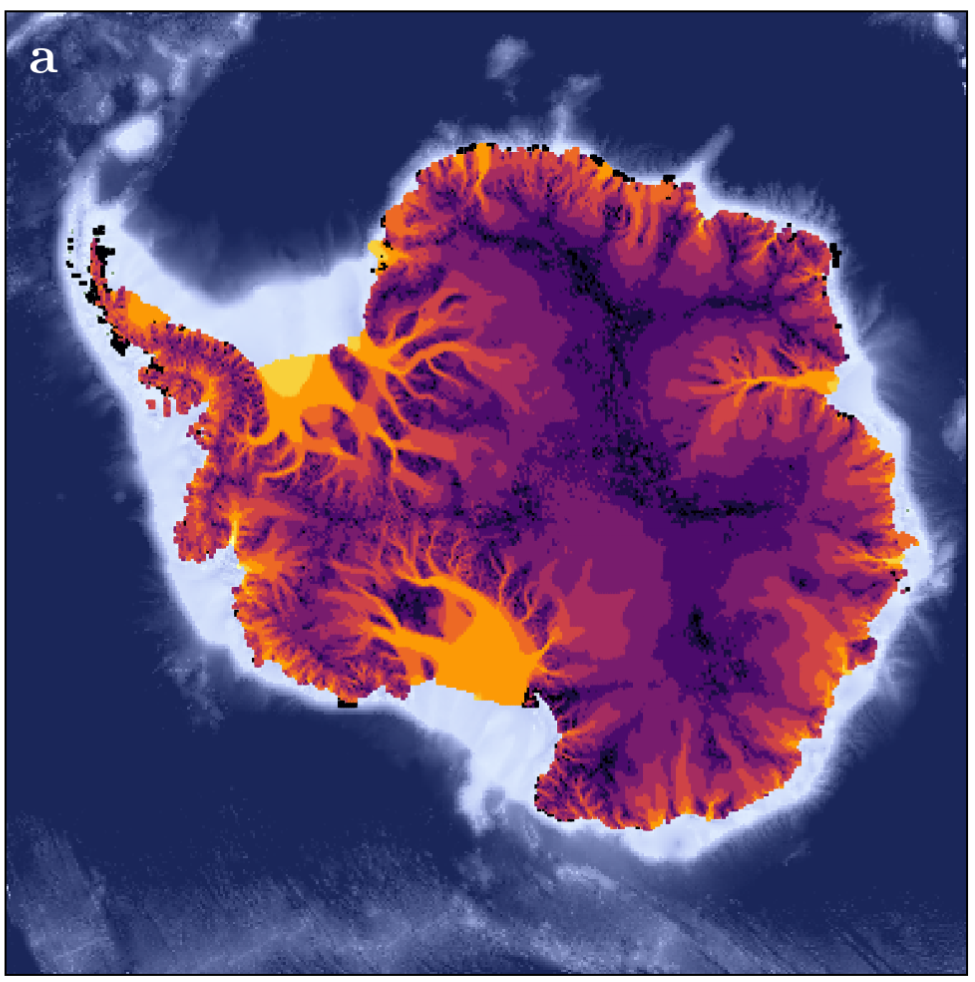
\includegraphics[width=0.95\textwidth]{figs/Fig-Antarctica-surface-velocity-nolegend.png}
            %\credit{Jan Swierczek-Jereczek}{2pt}
        \end{column}    
    \end{columns}

\hspace{5em}%\textbf{So, why make approximations?}

\vspace{0.3cm}

\hspace{50pt}
%$\bullet$ Computational cost
\hspace{10pt}
%$\bullet$ Processes
\hspace{10pt}
%$\bullet$ Scales

\end{frame}

\begin{frame}[t]{Motivation}

    \hspace{2em}The \textbf{momentum balance} of all of these systems \\ 
    \hspace{2em}can be described by the 
    \textbf{Navier-Stokes equations}. 

    \begin{columns}
        \begin{column}{0.32\textwidth}
            \centering
            \hspace{2em}\textbf{Atmosphere}
            \vspace{0.2cm} \newline
            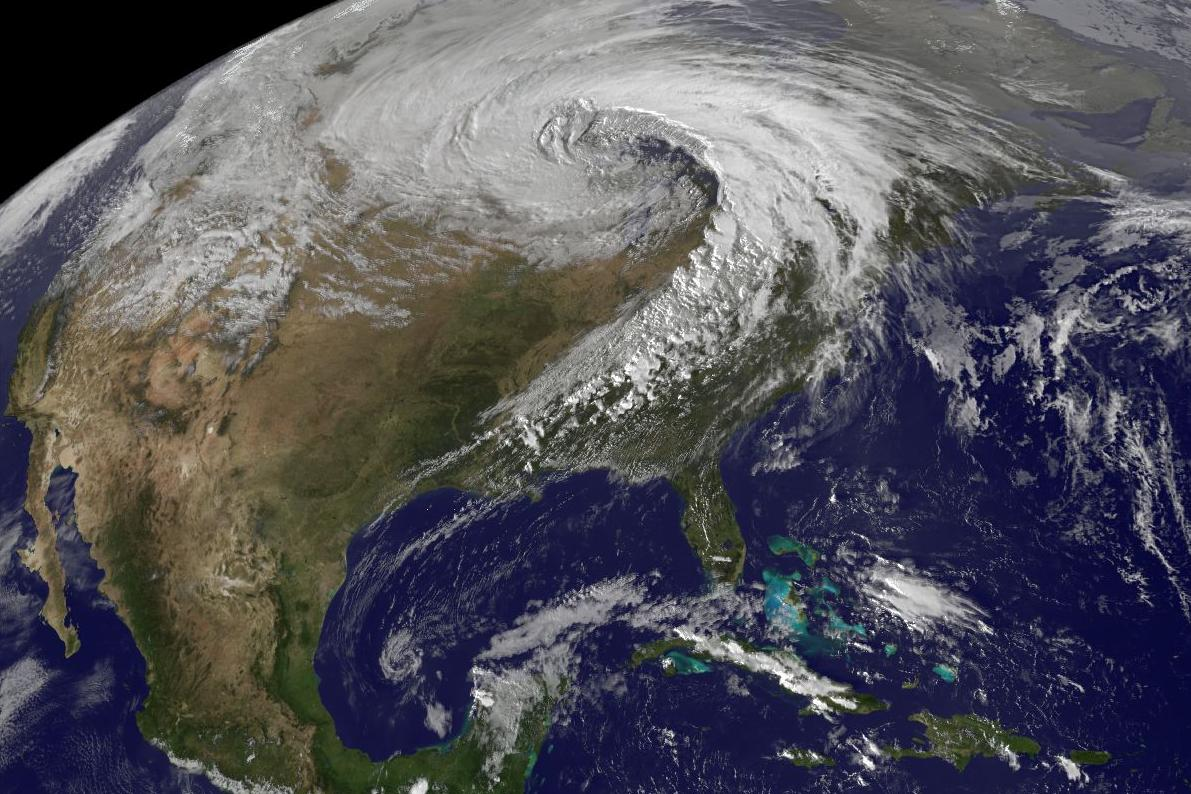
\includegraphics[width=0.9\textwidth]{figs/Fig-MidLatCyclone_2010-10-26_low_pressure.jpg}
            \credit{NOAA}{5pt}
        \end{column}
        \begin{column}{0.36\textwidth}
            \centering
            \hspace{2em}\textbf{Ocean}
            \vspace{0.2cm} \newline
            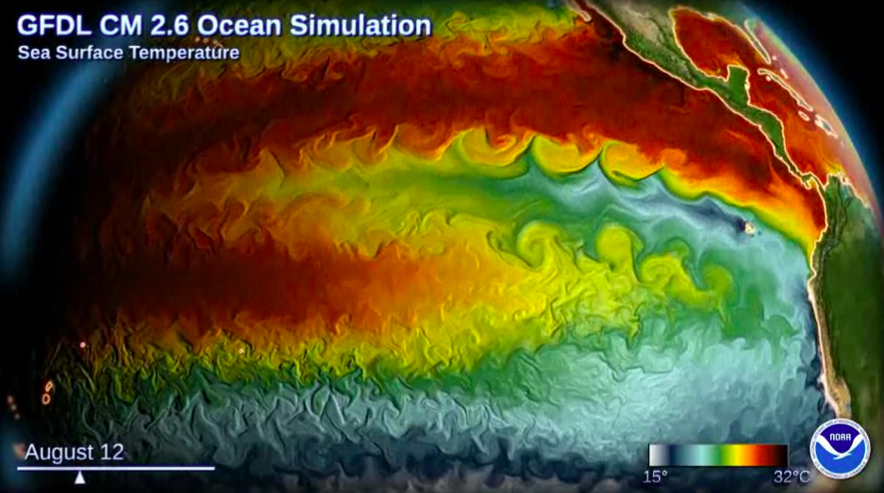
\includegraphics[width=0.9\textwidth]{figs/Fig-cm2.6-mesoscale-eddies.png}
            \credit{NOAA}{3pt}
        \end{column}
        \begin{column}{0.32\textwidth}
            \centering
            \hspace{2em}\textbf{Ice sheets}
            \vspace{0.2cm} \newline
            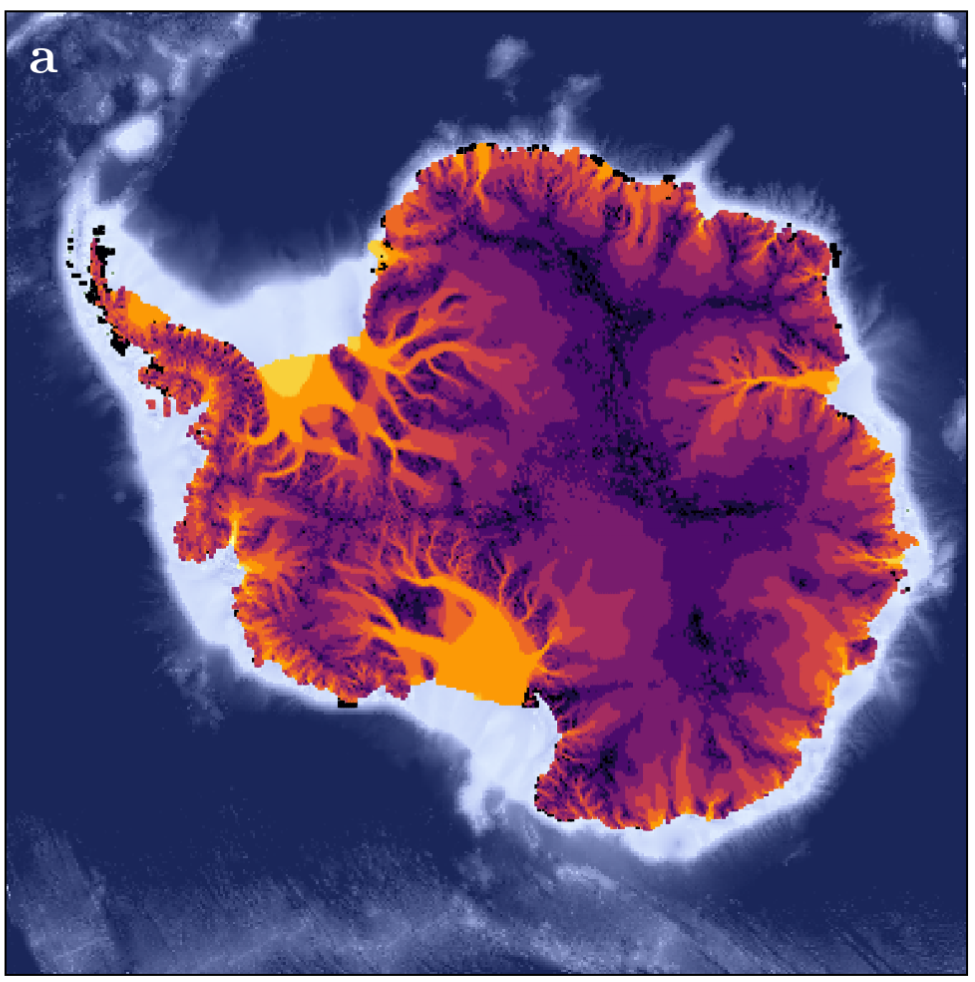
\includegraphics[width=0.95\textwidth]{figs/Fig-Antarctica-surface-velocity-nolegend.png}
            %\credit{Jan Swierczek-Jereczek}{2pt}
        \end{column}    
    \end{columns}

\hspace{5em}\textbf{So, why make approximations?}

\vspace{0.3cm}

\hspace{50pt}
$\bullet$ Computational cost
\hspace{10pt}
$\bullet$ Processes
\hspace{10pt}
$\bullet$ Scales

\end{frame}

\begin{frame}{Outline}
    \begin{columns}
    \begin{column}{0.15\textwidth}
    \end{column}
    \begin{column}{0.8\textwidth}
    \begin{enumerate}
        \item Rotation and spherical coordinates
        \item Navier-Stokes equations for a rotating frame of reference
        \item Scale analysis
        \item Atmosphere and ocean dynamics
        \begin{itemize}
            \item Shallow approximation
            \item Hydrostatic approximation
            \item Geostrophic approximation
            \item Boussinesq approximation (ocean)
        \end{itemize}
        \item Ice dynamics
        \begin{itemize}
            \item Blatter-Pattyn approximation
            \item Shallow shelf approximation
            \item Shallow ice approximation
        \end{itemize}
        \item Summary
    \end{enumerate}
    \end{column}
    \begin{column}{0.1\textwidth}
    \end{column}
    \end{columns}
\end{frame}

% SET THIS FRAME WITH DIFFERENT BACKGROUND
{\setbeamercolor{background canvas}{bg=mylightgray}

\begin{frame}{Rotation: Coriolis and Centrifugal force}
\begin{columns}
    \begin{column}{0.5\textwidth}
        \begin{center}
        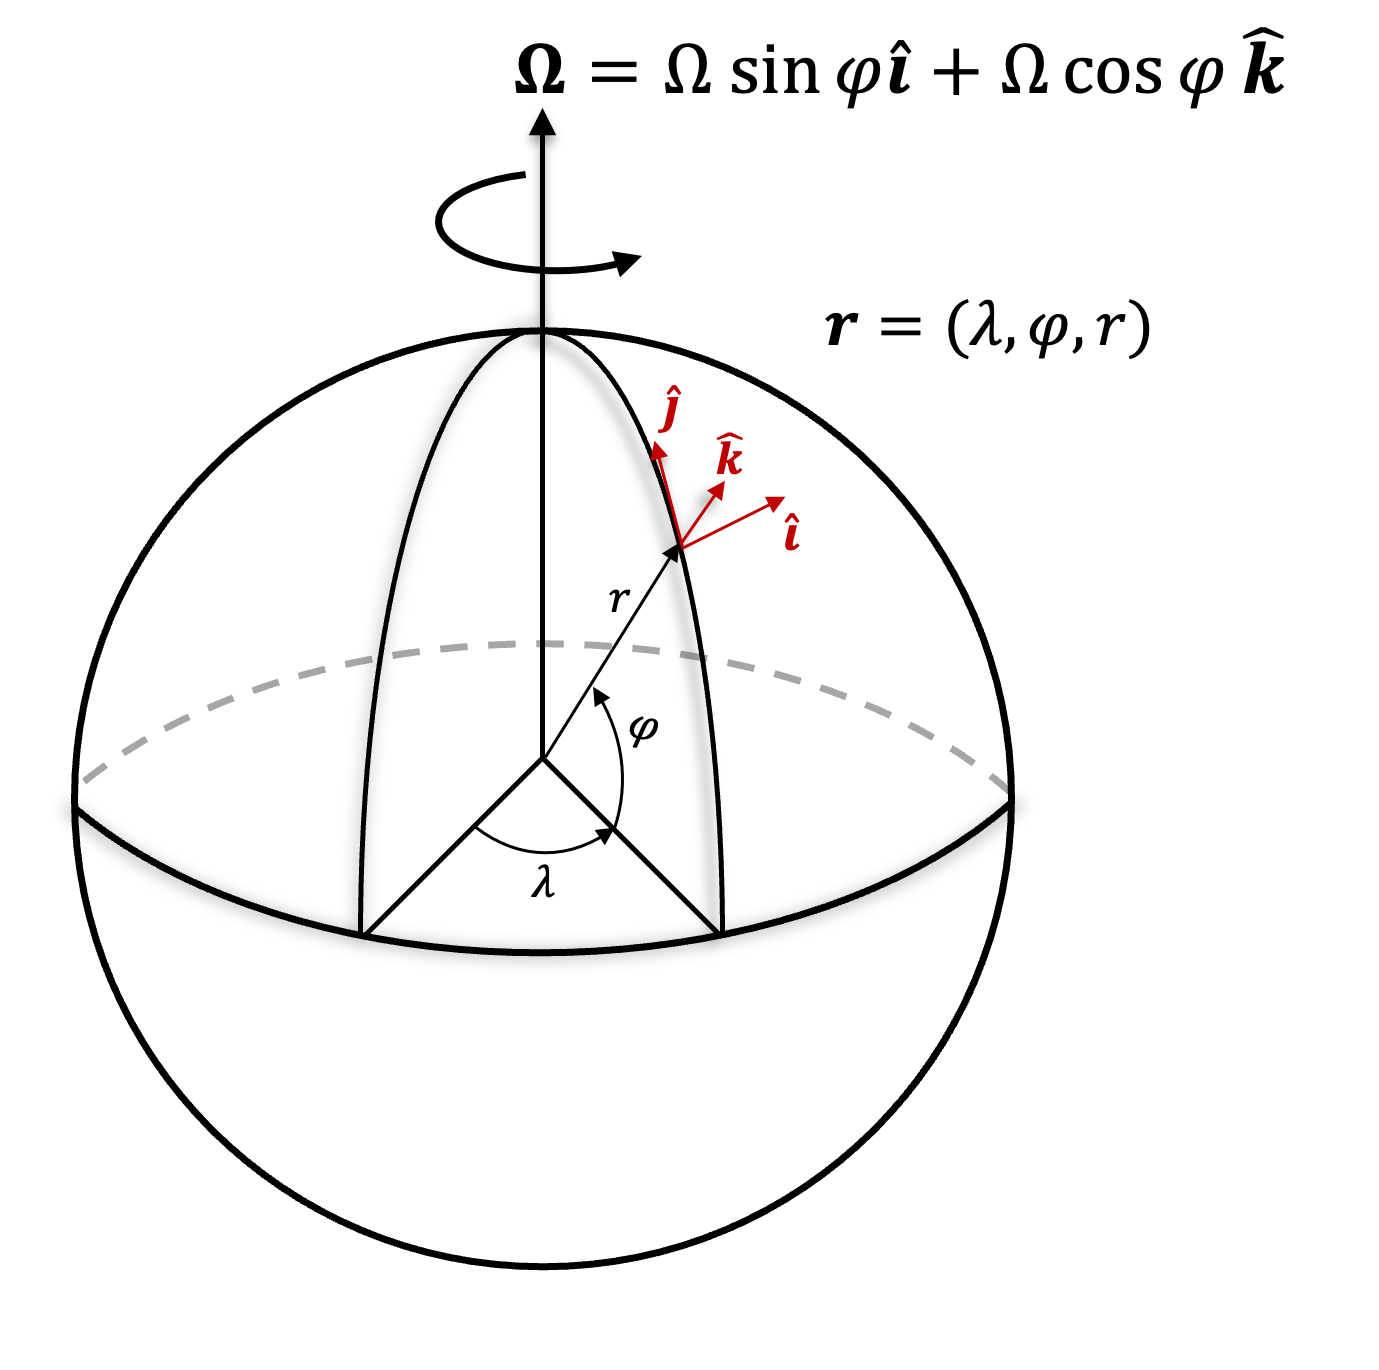
\includegraphics[width=0.8\textwidth]{figs/Fig-SphericalCoordRotating.png}
        \end{center}

        \vspace{-1em}

        \begin{minipage}{0.7\textwidth}
        \begin{block}{}
        \small
        Coriolis parameter: $f = 2\Omega \sin\phi$
        \end{block}
        \end{minipage}
        
    \end{column}
    \begin{column}{0.5\textwidth}
        The Earth revolves around its axis at the rate $\Omega = 7.2921\times10^{-5}$\,rad/s, so fluids at the surface operate in a rotating frame of reference.
        
        \vspace{1.2em}
        
        Coriolis and Centrifugal forces are known as \textbf{\emph{apparent forces}} --
        they only exist because the
        reference frame is in motion.
        
        \vspace{1.2em}
        
        The \textbf{Coriolis force} \emph{deflects} fluid
        parcels as a consequence of the
        Earth’s rotation.
        
        \vspace{1.2em}
        
        The \textbf{Centrifugal force} attempts to push fluid parcels away from the axis of rotation, but it is very small compared to gravity.
    \end{column}
\end{columns}
\end{frame}
} % end grey background color

\begin{frame}{Full Navier-Stokes equations}

We can start with the most general case of the Navier-Stokes equations, defined for a rotating frame of reference.

\begin{align*}
&\text{Momentum:} \quad 
\frac{D\mathbf{u}}{Dt} + 2\boldsymbol{\Omega} \times \mathbf{u}
= -\frac{1}{\rho}\nabla p + \nabla \Phi + \mathcal{F}\\
&\text{Continuity:} \quad 
\pdv{\rho}{t} + \nabla \cdot (\rho \mathbf{u}) = 0 \\
\end{align*}

\begin{columns}
    \begin{column}{0.15\textwidth}
    \end{column}
    \begin{column}{0.4\textwidth}
        $\mathbf{u}$: Velocity, $\mathbf{u} = (u,v,w)$ \\
        $p$: Pressure \\
        $\rho$: Density \\
        $\Phi = gz$: Gravitational potential \\
        $\mathcal{F}$: Frictional/dissipative forces \\
    \end{column}
    \begin{column}{0.3\textwidth}
        \begin{block}{}
        \centering
        \small{Recall definition of \\ 
        total derivative:} \\
        \vspace{0.1cm}
        $\frac{D\boldsymbol{u}}{Dt} = \pdv{\mathbf{u}}{t} + \mathbf{u} \cdot \nabla \mathbf{u}$
        \end{block}
    \end{column}
    \begin{column}{0.15\textwidth}
    \end{column}
\end{columns}

\vspace{0.3cm}

\end{frame}

\begin{frame}{Full Navier-Stokes equations}

\centering

\begin{table}[h!]
\centering
\begin{tabular}{cccccc}
\textcolor{red}{
$\displaystyle \frac{D\mathbf{u}}{Dt}$
}
&
\textcolor{blue}{
$\displaystyle +\,\, 2\boldsymbol{\Omega} \times \mathbf{u}$
}
&
$\displaystyle =$
&
\textcolor{teal}{
$\displaystyle -\frac{1}{\rho} \nabla p$
}
&
\textcolor{orange}{
$\displaystyle +\, \nabla \Phi$
}
&
\textcolor{purple}{
$\displaystyle +\, \mathcal{F}$
}
\\
\textcolor{red}{Inertia}
&
\textcolor{blue}{Rotation}
&
\,
&
\textcolor{teal}{\shortstack{Pressure \\ gradient}}
&
\textcolor{orange}{Gravity}
&
\textcolor{purple}{\shortstack{Friction/\\Dissipation}}
\end{tabular}
\end{table}

\end{frame}

% NAVIER-STOKES BY COMPONENT %%%%

\begin{frame}{Full Navier-Stokes equations by component*}
\vspace{0em}
\hspace{10cm}
{\small *\emph{in spherical coordinates}}

\begin{align*}
    &\textcolor{red}{    \frac{Du}{Dt}   }&
    &\textcolor{cyan}{   - \frac{uv \tan\phi}{r} + \frac{uw}{r}  }& 
    & \textcolor{blue}{   - 2\Omega v \sin\phi + 2\Omega w \cos\phi   }&
    & = &
    &\textcolor{teal}{   -\frac{1}{\rho r \cos\phi}\frac{\partial p}{\partial \lambda}  }&
    &&
    & \textcolor{purple}{\quad + \mathcal{F}_x }&
    \\
    &\textcolor{red}{    \frac{Dv}{Dt}   } &
    &\textcolor{cyan}{   + \frac{u^2 \tan\phi}{r} + \frac{vw}{r}     }&
    & \textcolor{blue}{   + 2\Omega u \sin\phi    }&
    & = &
    &\textcolor{teal}{   -\frac{1}{\rho r}\frac{\partial p}{\partial \phi}  }&
    &&
    & \textcolor{purple}{\quad + \mathcal{F}_y }&
    \\
    &\textcolor{red}{    \frac{Dw}{Dt}   } &
    &\textcolor{cyan}{   - \frac{u^2 + v^2}{r}   }&
    & \textcolor{blue}{   + 2\Omega u \cos\phi    }&
    & = &
    &\textcolor{teal}{   -\frac{1}{\rho}\frac{\partial p}{\partial z} }&
    & \textcolor{orange}{- g \quad}&
    & \textcolor{purple}{\quad + \mathcal{F}_z }&
\end{align*}

\begin{columns}
    \begin{column}{0.6\textwidth}
    \end{column}
    \begin{column}{0.4\textwidth}
        \begin{flushright}
            \vspace{-2em}
            {\footnotesize 
            \textcolor{red}{Inertia} \\
            \textcolor{cyan}{Curvature} \\
            \textcolor{blue}{Coriolis} \\
            \textcolor{teal}{Pressure gradient} \\
            \textcolor{orange}{Gravity} \\
            \textcolor{purple}{Friction/Dissipation}
            }
        \end{flushright}
    \end{column}
\end{columns}
        
\end{frame}

\begin{frame}{Full Navier-Stokes equations by component*}
\vspace{0em}
\hspace{10cm}
{\small *\emph{in spherical coordinates}}

\begin{align*}
    &\textcolor{red}{    \frac{Du}{Dt}   }&
    &\textcolor{cyan}{   - \frac{uv \tan\phi}{r} + \frac{uw}{r}  }& 
    & \textcolor{blue}{   - 2\Omega v \sin\phi + 2\Omega w \cos\phi   }&
    & = &
    &\textcolor{teal}{   -\frac{1}{\rho r \cos\phi}\frac{\partial p}{\partial \lambda}  }&
    &&
    & \textcolor{purple}{\quad + \mathcal{F}_x }&
    \\
    &\textcolor{red}{    \frac{Dv}{Dt}   } &
    &\textcolor{cyan}{   + \frac{u^2 \tan\phi}{r} + \frac{vw}{r}     }&
    & \textcolor{blue}{   + 2\Omega u \sin\phi    }&
    & = &
    &\textcolor{teal}{   -\frac{1}{\rho r}\frac{\partial p}{\partial \phi}  }&
    &&
    & \textcolor{purple}{\quad + \mathcal{F}_y }&
    \\
    &\textcolor{red}{    \frac{Dw}{Dt}   } &
    &\textcolor{cyan}{   - \frac{u^2 + v^2}{r}   }&
    & \textcolor{blue}{   + 2\Omega u \cos\phi    }&
    & = &
    &\textcolor{teal}{   -\frac{1}{\rho}\frac{\partial p}{\partial z} }&
    & \textcolor{orange}{- g \quad}&
    & \textcolor{purple}{\quad + \mathcal{F}_z }&
\end{align*}

\begin{columns}
    \begin{column}{0.6\textwidth}
    Equations have many terms, how can they be simplified?

    \vspace{0.5em}
    
    \hspace{5em}\textbf{\myarrow[scale=1.5] Scale analysis}
    \end{column}
    \begin{column}{0.4\textwidth}
        \begin{flushright}
            \vspace{-2em}
            {\footnotesize 
            \textcolor{red}{Inertia} \\
            \textcolor{cyan}{Curvature} \\
            \textcolor{blue}{Coriolis} \\
            \textcolor{teal}{Pressure gradient} \\
            \textcolor{orange}{Gravity} \\
            \textcolor{purple}{Friction/Dissipation}
            }
        \end{flushright}
    \end{column}
\end{columns}
        
\end{frame}

\begin{frame}{Scale analysis}
    \begin{center}
    \begin{minipage}[t]{0.6\textwidth}
    \begin{block}{Scaling terms}
        \vspace{-1.2em}
        \begin{align*}
            L \quad & \text{Horizontal distance scale} \\
            U \quad & \text{Horizontal velocity scale} \\
            T \quad & \text{Time scale }(T=L/U) \\
            H \quad & \text{Vertical distance scale} \\
            W \quad & \text{Vertical velocity scale} \\
            \Delta P/\rho \quad & \text{Horizontal pressure fluctuation scale}
        \end{align*}
    \end{block}
    \end{minipage}
    \end{center}
    
    \vspace{2em}
    
    The material derivative $\frac{D}{Dt}$ represents change on the time-scale of motion.

    So, its scale is represented as $\left[\frac{D}{Dt}\right]=\frac{1}{T}=\frac{U}{L}$
\end{frame}

% EXTRA DEFINITIONS: Reynolds Number, Rossby Number

\begin{frame}[t]{Some measures of scale}

\vspace{3em}

\begin{columns}
    \begin{column}[t]{0.5\textwidth}
        {\small
        The \boldblue{Reynolds number (Re)} is a dimensionless number that characterizes the relative importance of inertial forces to viscous forces in a fluid flow.
        \vspace{-0.5em}
        \begin{align*}
            \text{Re} = \frac{U L}{\nu} = \frac{\text{inertial forces}}{\text{viscous forces}}
        \end{align*}

        % \begin{itemize}
        %     \item \boldmath{$\text{Re} > 1000$}: Inertial forces dominate, flow becomes turbulent, with eddies and chaotic motion (e.g. atmospheric winds, ocean currents).
        %     \item \boldmath{$\text{Re} < 1$}: Viscous forces dominate, flow is smooth, laminar, and very orderly (e.g. ice sheets).
        % \end{itemize}
        }
    \end{column}
    \begin{column}[t]{0.5\textwidth}
        {\small
        Meanwhile, the \boldblue{Rossby number (Ro)} tells us about the relative importance of the Coriolis force.
        \vspace{-0.2em}
        \begin{align*}
        \text{Ro} = \frac{U}{fL} = \ 
        \frac{\text{inertial forces}}
        {\text{Coriolis force}}
        \end{align*}

        % \begin{itemize}
        %     \item \boldmath{$\text{Ro} \gg 1$}: Coriolis force is negligible, inertia dominates (e.g., thunderstorms).
        %     \item \boldmath{$\text{Ro} \sim 1$}: Coriolis and inertia are both important (e.g., mesoscale ocean eddies).
        %     \item \boldmath{$\text{Ro} \ll 1$}: Coriolis force dominates over inertia, and the flow is in \emph{geostrophic balance} (e.g., large-scale ocean or atmospheric flow).
        % \end{itemize}
        }
    \end{column}
\end{columns}
\end{frame}

\begin{frame}[t]{Scaling examples}

\begin{columns}
    \begin{column}[t]{0.5\textwidth}
        \centering
        \textbf{Mid-latitude storms}
        \vspace{0.2cm}

        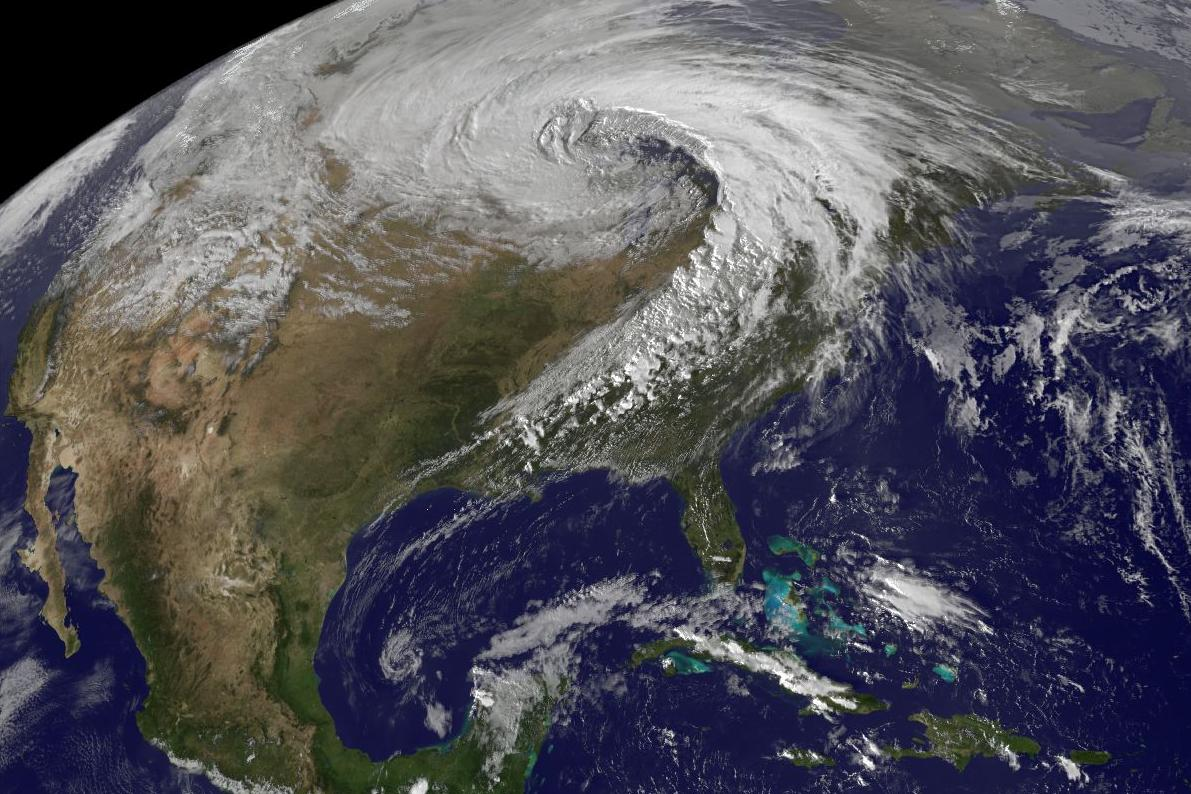
\includegraphics[width=0.7\textwidth]{figs/Fig-MidLatCyclone_2010-10-26_low_pressure.jpg}
        \credit{NOAA}{25pt}
        
        \vspace{0.5em}
        
         $U\sim10-20$\,m/s, \hspace{10pt}
        $L\sim1000-2000$\,km \\
        $f\sim10^{-4}$\,s$^{-1}$, \hspace{10pt} 
        $\nu = 10^{-5}$\,m$^2$s${-1}$\\
        
        {\boldmath
        \begin{align*}
            \text{Re}\sim10^{8}, \hspace{10pt}
            \text{Ro}\sim0.1-1 \\
        \end{align*}
        }
        
    \end{column}
    \begin{column}[t]{0.5\textwidth}
        \centering
        \textbf{Oceanic mesoscale eddies}
        \vspace{0.2cm}
        
        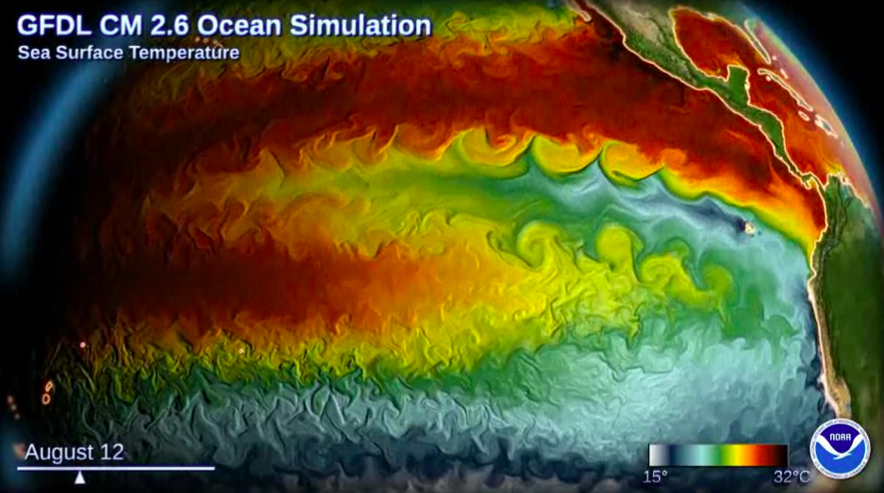
\includegraphics[width=0.8\textwidth]{figs/Fig-cm2.6-mesoscale-eddies.png}
        \credit{NOAA}{15pt}

        \vspace{1.0em}

         \begin{small}
        $U\sim0.1-1$\,m/s, \hspace{10pt}
        $L\sim10-100$\,km \\
        $f\sim10^{-4}$\,s$^{-1}$, \hspace{10pt} 
        $\nu = 10^{-6}$\,m$^2$s${-1}$\\
        \end{small}

        {\boldmath
        \begin{align*}
            \text{Re}\sim10^{7}, \hspace{10pt}
            \text{Ro}\sim0.1-1 \\
        \end{align*}
        }
        
    \end{column}
    
\end{columns}

\end{frame}

\begin{frame}[t]{Scaling examples}

        \centering
        
        \textbf{Ice sheets}
        
        \vspace{1.0em}

        \begin{columns}
            \begin{column}{0.5\textwidth}
                \hfill
                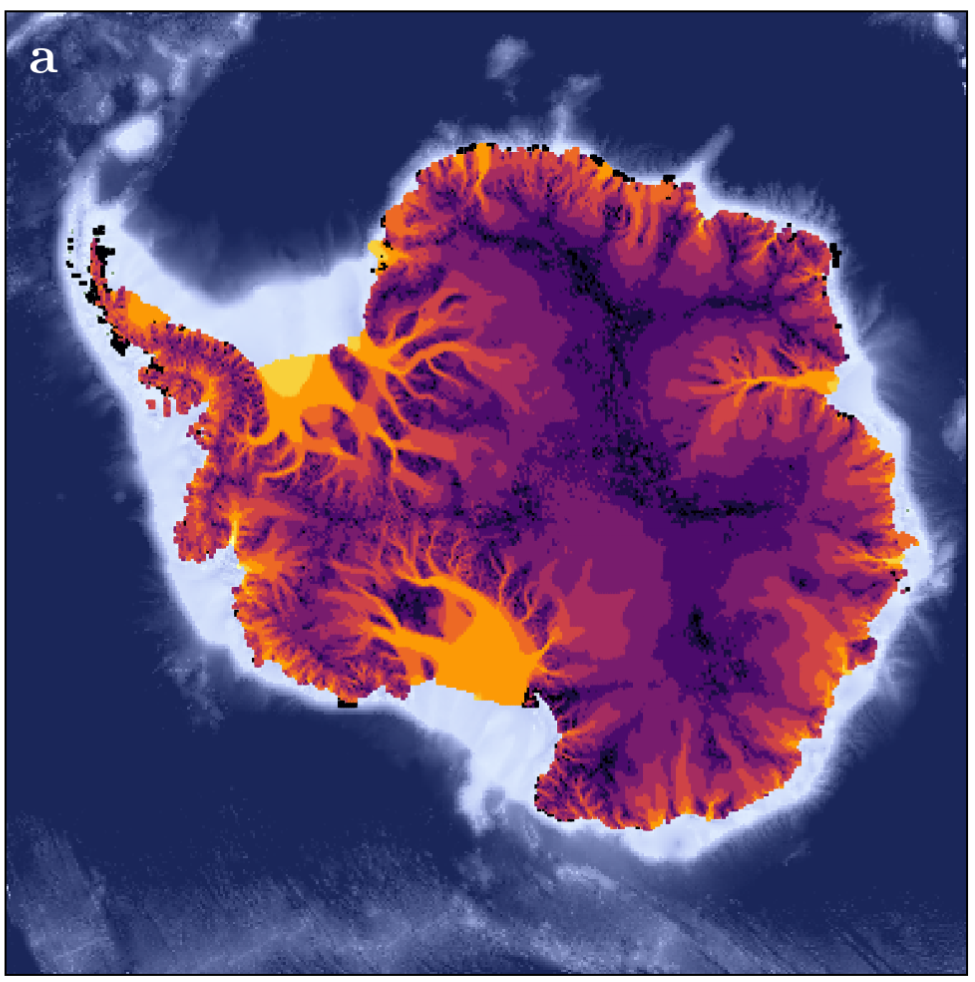
\includegraphics[width=0.7\textwidth]{figs/Fig-Antarctica-surface-velocity-nolegend.png}
                %\credit{Jan Swierczek-Jereczek}{-5pt}
            \end{column}
            \begin{column}{0.4\textwidth}
                \vspace{3em}
                
                $U\sim1-1000$\,m/yr$\quad < 10^{-4}$\,m/s \\
                $L\sim10^3-10^6$\,m \\
                $\nu\sim 10^{10}-10^{12}$\,m$^2$s$^{-1}$
                
                {\boldmath
                \begin{align*}
                    \text{Re}\sim10^{-11}
                \end{align*}
                }

            \end{column}
        \end{columns}

\end{frame}

\begin{frame}{}

\centering

{\huge 
Atmosphere and Ocean Dynamics
}

\end{frame}

\begin{frame}{Full Navier-Stokes equations by component*}
\vspace{0em}
\hspace{10cm}
{\small *\emph{in spherical coordinates}}

\begin{align*}
    &\textcolor{red}{    \frac{Du}{Dt}   }&
    &\textcolor{cyan}{   - \frac{uv \tan\phi}{r} + \frac{uw}{r}  }& 
    & \textcolor{blue}{   - 2\Omega v \sin\phi + 2\Omega w \cos\phi   }&
    & = &
    &\textcolor{teal}{   -\frac{1}{\rho r \cos\phi}\frac{\partial p}{\partial \lambda}  }&
    &&
    & \textcolor{purple}{\quad + \mathcal{F}_x }&
    \\
    &\textcolor{red}{    \frac{Dv}{Dt}   } &
    &\textcolor{cyan}{   + \frac{u^2 \tan\phi}{r} + \frac{vw}{r}     }&
    & \textcolor{blue}{   + 2\Omega u \sin\phi    }&
    & = &
    &\textcolor{teal}{   -\frac{1}{\rho r}\frac{\partial p}{\partial \phi}  }&
    &&
    & \textcolor{purple}{\quad + \mathcal{F}_y }&
    \\
    &\textcolor{red}{    \frac{Dw}{Dt}   } &
    &\textcolor{cyan}{   - \frac{u^2 + v^2}{r}   }&
    & \textcolor{blue}{   + 2\Omega u \cos\phi    }&
    & = &
    &\textcolor{teal}{   -\frac{1}{\rho}\frac{\partial p}{\partial z} }&
    & \textcolor{orange}{- g \quad}&
    & \textcolor{purple}{\quad + \mathcal{F}_z }&
\end{align*}

\begin{columns}
    \begin{column}{0.6\textwidth}
    \end{column}
    \begin{column}{0.4\textwidth}
        \begin{flushright}
            \vspace{-2em}
            {\footnotesize 
            \textcolor{red}{Inertia} \\
            \textcolor{cyan}{Curvature} \\
            \textcolor{blue}{Coriolis} \\
            \textcolor{teal}{Pressure gradient} \\
            \textcolor{orange}{Gravity} \\
            \textcolor{purple}{Friction/Dissipation}
            }
        \end{flushright}
    \end{column}
\end{columns}
        
\end{frame}

\begin{frame}[t]{Atmospheric and ocean dynamics}
\vspace{0em}
\hspace{10cm}
{\small \,\,}


\begin{align*}
    &\textcolor{red}{    \frac{Du}{Dt}   }&
    &\textcolor{cyan}{   - \frac{uv \tan\phi}{r} + \frac{uw}{r}  }& 
    & \textcolor{blue}{   - 2\Omega v \sin\phi + 2\Omega w \cos\phi   }&
    & = &
    &\textcolor{teal}{   -\frac{1}{\rho r \cos\phi}\frac{\partial p}{\partial \lambda}  }&
    &&
    & \textcolor{purple}{\quad + \nu \nabla^2 u }&
    \\
    &\textcolor{red}{    \frac{Dv}{Dt}   } &
    &\textcolor{cyan}{   + \frac{u^2 \tan\phi}{r} + \frac{vw}{r}     }&
    & \textcolor{blue}{   + 2\Omega u \sin\phi    }&
    & = &
    &\textcolor{teal}{   -\frac{1}{\rho r}\frac{\partial p}{\partial \phi}  }&
    &&
    & \textcolor{purple}{\quad + \nu \nabla^2 v }&
    \\
    &\textcolor{red}{    \frac{Dw}{Dt}   } &
    &\textcolor{cyan}{   - \frac{u^2 + v^2}{r}   }&
    & \textcolor{blue}{   + 2\Omega u \cos\phi    }&
    & = &
    &\textcolor{teal}{   -\frac{1}{\rho}\frac{\partial p}{\partial z} }&
    & \textcolor{orange}{- g \quad}&
    & \textcolor{purple}{\quad + \nu \nabla^2 w }&
\end{align*}

\begin{columns}
    \begin{column}{0.7\textwidth}
    \end{column}
    \begin{column}{0.3\textwidth}
        \begin{block}{}
            {\footnotesize
            Viscous momentum diffusion \\
            in a Newtonian fluid:
            }
            \begin{center}
            {\small
            $\mathcal{F}\rightarrow\nu\nabla^2\mathbf{u} $
            }
            \end{center}
        \end{block}

    \end{column}
\end{columns}
        
\end{frame}

\begin{frame}[t]{Atmospheric and ocean dynamics}

\vspace{-1.0em}

\begin{center}
\textbf{{\large
Shallow atmosphere/ocean approximation
}}
\end{center}

\begin{columns}
    \begin{column}[t]{0.6\textwidth}

        First, given the radius of the Earth $a=6370$\,km, \\and that $z \ll a$ in the atmosphere and ocean, we \\can assume a constant radius
        \begin{columns}
            \begin{column}{0.6\textwidth}
                \begin{align*}
                    r=a=\text{const}
                \end{align*}
                And then
                \begin{align*}
                    \frac{\partial}{\partial r} = \frac{\partial z}{\partial r}\frac{\partial}{\partial z} \simeq \frac{\partial}{\partial z}
                \end{align*}
            \end{column}
            \begin{column}{0.4\textwidth}
                \vspace{3em}
                \begin{block}{}
                    \small
                    Recall for spherical coordinates:
                    \begin{align*}
                    &dx = r \cos\phi d\lambda \\
                    &dy = r\, d\phi
                    \end{align*}
                \end{block}
            \end{column}
        \end{columns}
    \end{column}
    \begin{column}[t]{0.4\textwidth}
        \begin{center}
        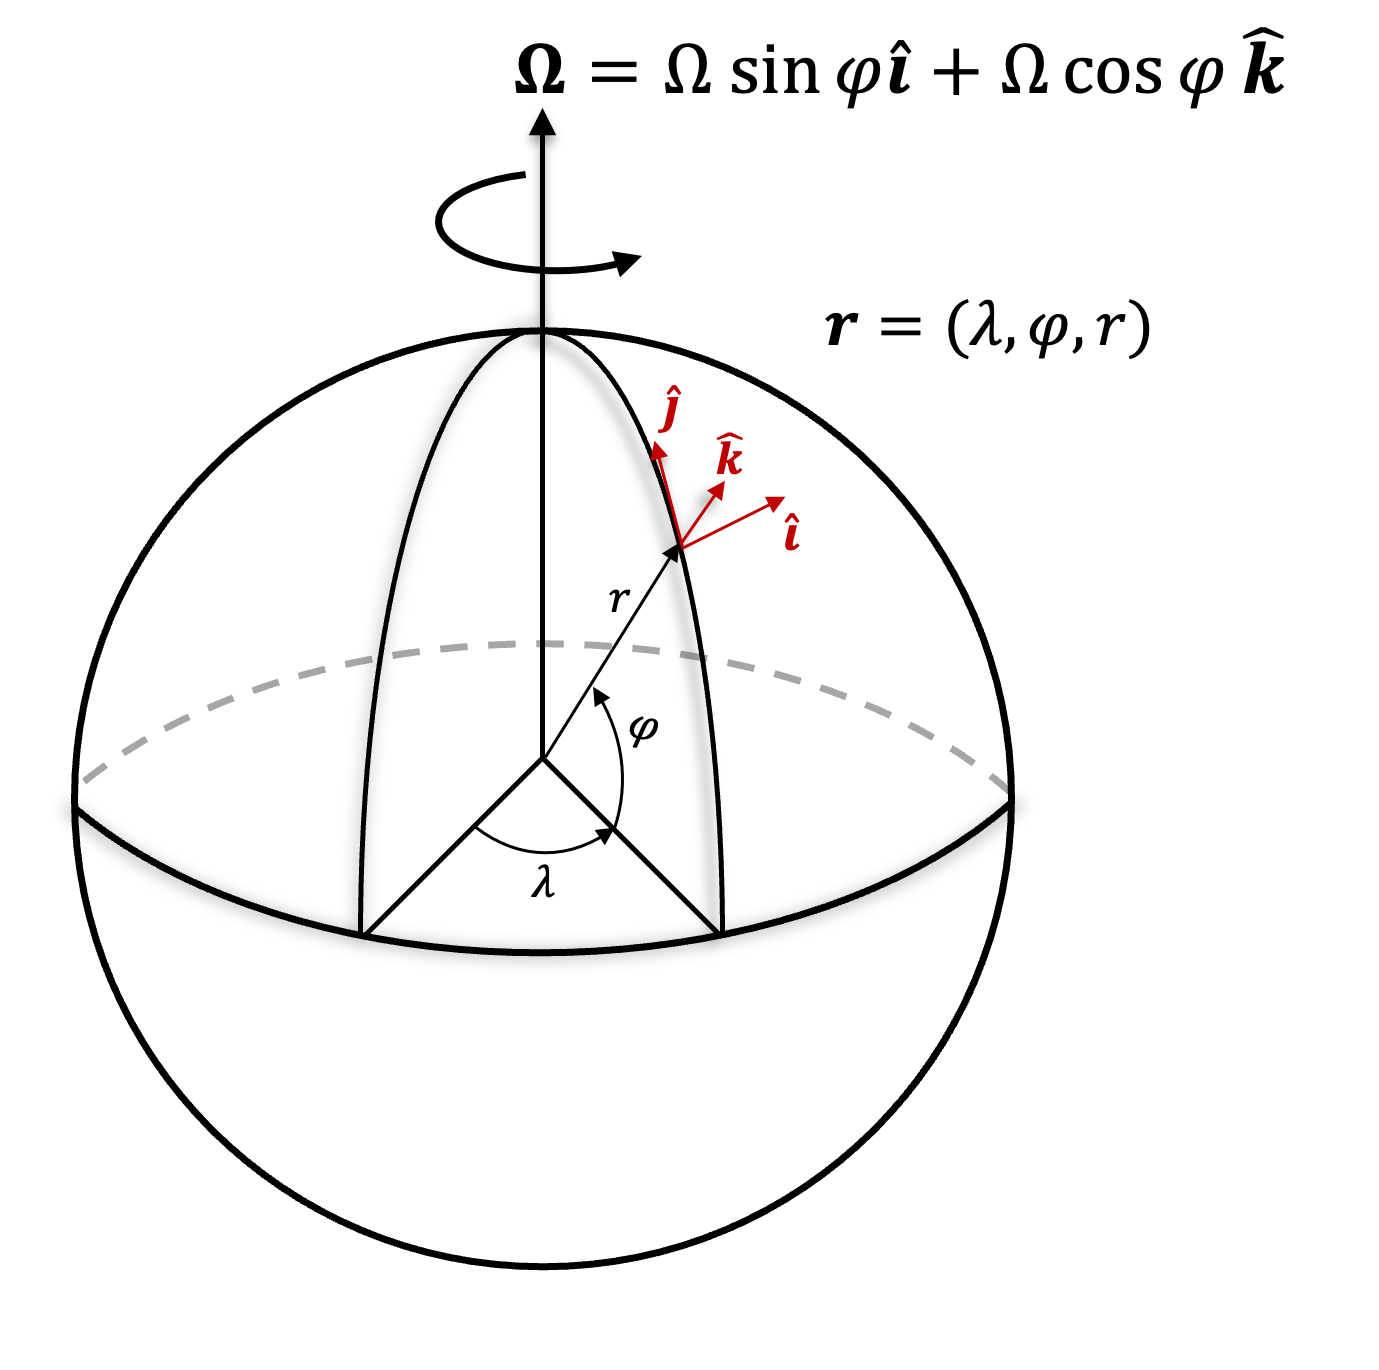
\includegraphics[width=0.8\textwidth]{figs/Fig-SphericalCoordRotating.png}
         \end{center}         
    \end{column}
\end{columns}

\end{frame}

\begin{frame}[t]{Atmospheric and ocean dynamics}

\vspace{-1.0em}

\begin{center}
\textbf{{\large
Shallow atmosphere/ocean approximation
}}
\end{center}

\begin{align*}
    &\textcolor{red}{    \frac{Du}{Dt}   }&
    &\textcolor{cyan}{   - \frac{uv \tan\phi}{a} + \frac{uw}{a}  }& 
    & \textcolor{blue}{   - 2\Omega v \sin\phi + 2\Omega w \cos\phi   }&
    & = &
    &\textcolor{teal}{   -\frac{1}{\rho}\frac{\partial p}{\partial x}  }&
    &&
    & \textcolor{purple}{\quad + \nu \nabla^2 u }&
    \\
    &\textcolor{red}{    \frac{Dv}{Dt}   } &
    &\textcolor{cyan}{   + \frac{u^2 \tan\phi}{a} + \frac{vw}{a}     }&
    & \textcolor{blue}{   + 2\Omega u \sin\phi    }&
    & = &
    &\textcolor{teal}{   -\frac{1}{\rho}\frac{\partial p}{\partial y}  }&
    &&
    & \textcolor{purple}{\quad + \nu \nabla^2 v }&
    \\
    &\textcolor{red}{    \frac{Dw}{Dt}   } &
    &\textcolor{cyan}{   - \frac{u^2 + v^2}{a}   }&
    & \textcolor{blue}{   + 2\Omega u \cos\phi    }&
    & = &
    &\textcolor{teal}{   -\frac{1}{\rho}\frac{\partial p}{\partial z} }&
    & \textcolor{orange}{- g \quad}&
    & \textcolor{purple}{\quad + \nu \nabla^2 w }&
\end{align*}

\begin{columns}
    \begin{column}{0.7\textwidth}
    \end{column}
    \begin{column}{0.3\textwidth}
        \begin{block}{}
            {\footnotesize
            Viscous momentum diffusion \\
            in a Newtonian fluid:
            }
            \begin{center}
            {\small
            $\mathcal{F}\rightarrow\nu\nabla^2\mathbf{u} $
            }
            \end{center}
        \end{block}

    \end{column}
\end{columns}

\end{frame}

\begin{frame}[t]{Atmospheric and ocean dynamics}

\vspace{-1.0em}

\begin{center}
\textbf{{\large
Shallow atmosphere/ocean approximation
}}
\end{center}

\begin{align*}
    &\textcolor{red}{    \frac{Du}{Dt}   }&
    &\textcolor{cyan}{   - \frac{uv \tan\phi}{a} + \frac{uw}{a}  }& 
    & \textcolor{blue}{   - 2\Omega v \sin\phi + 2\Omega w \cos\phi   }&
    & = &
    &\textcolor{teal}{   -\frac{1}{\rho}\frac{\partial p}{\partial x}  }&
    &&
    & \textcolor{purple}{\quad + \nu \nabla^2 u }&
    \\
    &\textcolor{red}{    \frac{Dv}{Dt}   } &
    &\textcolor{cyan}{   + \frac{u^2 \tan\phi}{a} + \frac{vw}{a}     }&
    & \textcolor{blue}{   + 2\Omega u \sin\phi    }&
    & = &
    &\textcolor{teal}{   -\frac{1}{\rho}\frac{\partial p}{\partial y}  }&
    &&
    & \textcolor{purple}{\quad + \nu \nabla^2 v }&
    \\
    &\textcolor{red}{    \frac{Dw}{Dt}   } &
    &\textcolor{cyan}{   - \frac{u^2 + v^2}{a}   }&
    & \textcolor{blue}{   + 2\Omega u \cos\phi    }&
    & = &
    &\textcolor{teal}{   -\frac{1}{\rho}\frac{\partial p}{\partial z} }&
    & \textcolor{orange}{- g \quad}&
    & \textcolor{purple}{\quad + \nu \nabla^2 w }&
\end{align*}

\begin{columns}
    \begin{column}{0.7\textwidth}
        Can we eliminate some terms via scale analysis?
    \end{column}
    \begin{column}{0.3\textwidth}
        \begin{block}{}
            {\footnotesize
            Viscous momentum diffusion \\
            in a Newtonian fluid:
            }
            \begin{center}
            {\small
            $\mathcal{F}\rightarrow\nu\nabla^2\mathbf{u} $
            }
            \end{center}
        \end{block}

    \end{column}
\end{columns}

\end{frame}

\begin{frame}[t]{Atmospheric and ocean dynamics}

\vspace{-1.0em}

\begin{center}
\textbf{{\large
Atmospheric scale analysis for mid-latitude synoptic systems
}}
\end{center}

\footnotesize
\centering

\vspace{1.5em}

\begin{columns}
    \begin{column}{0.5\textwidth}
        % Note: values below from Holt (2004), Table 2.1 (p.39)
        \begin{align*}
            L &\sim 10^6\,\text{m} && \text{Horizontal distance scale} \\
            U &\sim 10\,\text{m s}^{-1} && \text{Horizontal velocity scale} \\
            T &\sim 10^5\,\text{s} && \text{Time scale } (T = L/U) \\
            H &\sim 10^4\,\text{m} && \text{Vertical distance scale} \\
            W &\sim 10^{-2}\,\text{m s}^{-1} && \text{Vertical velocity scale} \\
            \Delta P/\rho &\sim 10^3\,\text{m}^2\,\text{s}^{-2} && \text{Horizontal pressure} \\
            & && \quad\quad\quad \text{fluctuation scale}
        \end{align*}
    \end{column}
    \begin{column}{0.4\textwidth}
        \begin{align*}
            f_0 &= 10^{-4}\,\text{s}^{-1} && \text{Coriolis parameter} \\
            a &= 6370 \times 10^3\,\text{m} && \text{Radius of the Earth} \\
            \nu &= 10^{-5}\,\text{m}^2\,\text{s}^{-1} && \text{Kinematic viscosity} \\
            P_0 &= 10^{5}\,\text{Pa} && \text{Surface air pressure} \\
            \rho &\sim 1\,\text{kg}\,\text{m}^{-3} && \text{Density}
        \end{align*}
    \end{column}
\end{columns}

\end{frame}

% HYDROSTATIC APPROXIMATION
\begin{frame}[t]{Atmospheric and ocean dynamics}

\vspace{-1.0em}

\begin{center}
\textbf{{\large
Atmospheric scale analysis for mid-latitude synoptic systems
}}
\end{center}

\small 
\center 

\vspace{-0.5em}

Vertical equation

\begin{align*}
    &\textcolor{red}{    \frac{Dw}{Dt}   } &
    &\textcolor{cyan}{   - \frac{u^2 + v^2}{a}   }&
    &\textcolor{blue}{   + 2\Omega u \cos\phi    }&
    & = &
    &\textcolor{teal}{   -\frac{1}{\rho}\frac{\partial p}{\partial z} }&
    &\textcolor{orange}{- g \quad}&
    &\textcolor{purple}{\quad + \nu \nabla^2 w }&
    \\ \\
      &\textcolor{black}{   \frac{UW}{L}   } &
      &\textcolor{black}{   \quad\quad\frac{U^2}{a} }&
      &\textcolor{black}{\quad\quad f_0 U }&
      &&
      &\textcolor{black}{\,\,\,\,\,\frac{P_0} {\rho H}  }&
      &\textcolor{black}{  g    }&
      &\textcolor{black}{\quad\frac{\nu W}{H^2} }&
    \\ \\
      &\textcolor{black}{   10^{-7} }&
      &\textcolor{black}{\quad\quad10^{-5} }&
      &\textcolor{black}{\quad\quad10^{-3} }&
      &&
      &\textcolor{black}{\quad 10  }&
      &\textcolor{black}{10     }&
      &\textcolor{black}{\quad10^{-15}}&
\end{align*}

\end{frame}

% HYDROSTATIC APPROXIMATION

\begin{frame}[t]{Atmospheric and ocean dynamics}

\vspace{-1.0em}

\begin{center}
\textbf{{\large
Atmospheric scale analysis for mid-latitude synoptic systems
}}
\end{center}

\small 
\center 

\vspace{-0.5em}

Vertical equation

\begin{align*}
    &\textcolorg{red}{    \frac{Dw}{Dt}   } &
    &\textcolorg{cyan}{   - \frac{u^2 + v^2}{a}   }&
    &\textcolorg{blue}{   + 2\Omega u \cos\phi    }&
    & = &
    &\textcolor{teal}{   -\frac{1}{\rho}\frac{\partial p}{\partial z} }&
    &\textcolor{orange}{- g \quad}&
    &\textcolorg{purple}{\quad + \nu \nabla^2 w }&
    \\ \\
      &\textcolorg{black}{   \frac{UW}{L}   } &
      &\textcolorg{black}{   \quad\quad\frac{U^2}{a} }&
      &\textcolorg{black}{\quad\quad f_0 U }&
      &&
      &\textcolor{black}{\,\,\,\,\,\frac{P_0} {\rho H}  }&
      &\textcolor{black}{  g    }&
      &\textcolorg{black}{\quad\frac{\nu W}{H^2} }&
    \\ \\
      &\textcolorg{black}{   10^{-7} }&
      &\textcolorg{black}{\quad\quad10^{-5} }&
      &\textcolorg{black}{\quad\quad10^{-3} }&
      &&
      &\textcolor{black}{\quad 10  }&
      &\textcolor{black}{10     }&
      &\textcolorg{black}{\quad10^{-15}}&
\end{align*}

\end{frame}

% HYDROSTATIC APPROXIMATION %%%%%%%%%%%%%%%%%%%%%%%%%%%%%%%

\begin{frame}[t]{Atmospheric and ocean dynamics}

\vspace{-1.0em}

\begin{center}
\textbf{{\large
Hydrostatic approximation
}}
\end{center}

\small 
\center 

\vspace{-0.5em}

Vertical equation

\vspace{-0.5em}

{\normalsize
\begin{align*}
    \frac{\partial p}{\partial z} = -\rho g
\end{align*}
}

\begin{columns}
    \begin{column}{0.4\textwidth}
        The vertical momentum equation reduces to a balance between the \textbf{vertical pressure gradient} and \textbf{gravity}. This is known as the \boldblue{hydrostatic balance}.

        \vspace{0.5em}
        
        With this formulation, pressure $p(z)$ is determined by the weight of the fluid above the current height $z$.
    \end{column}
    \begin{column}{0.4\textwidth}
        Integrating from the top of the atmosphere downward, and noting that $p(z=\infty)=0$ then gives the pressure at any level $z$:
        \begin{align*}
            p(z) = g \int_z^\infty \rho dz
        \end{align*}
    \end{column}
\end{columns}
        
\end{frame}

\begin{frame}[t]{Atmospheric and ocean dynamics}

\vspace{-1.0em}

\begin{center}
\textbf{{\large
Atmospheric scale analysis for mid-latitude synoptic systems
}}
\end{center}

\small 
\center 

\vspace{-0.5em}

Horizontal equations

\begin{align*}
    &\textcolor{red}{    \frac{Du}{Dt}   }&
    &\textcolor{cyan}{   - \frac{uv \tan\phi}{a} }
     \textcolor{cyan}{  + \frac{uw}{a}  }& 
    & \textcolor{blue}{   - 2\Omega v \sin\phi }
     \textcolor{blue}{  \,+ 2\Omega w \cos\phi }&
    & = &
    &\textcolor{teal}{   -\frac{1}{\rho}\frac{\partial p}{\partial x}  }&
    & \textcolor{purple}{\quad + \nu \nabla^2 u }&
    \\
    &\textcolor{red}{    \frac{Dv}{Dt}   } &
    &\textcolor{cyan}{   + \frac{u^2 \tan\phi}{a} }
     \textcolor{cyan}{  + \frac{vw}{a}     }&
    & \textcolor{blue}{   + 2\Omega u \sin\phi    }&
    & = &
    &\textcolor{teal}{   -\frac{1}{\rho}\frac{\partial p}{\partial y}  }&
    & \textcolor{purple}{\quad + \nu \nabla^2 v }&
    \\ \\
      &\textcolor{black}{ \frac{U^2}{L}  }&
      &\textcolor{black}{ \quad \frac{U^2}{a} }
       \textcolor{black}{\quad\quad\quad\frac{UW}{a} }&
      &\textcolor{black}{ \quad\quad f_0 U      }
       \textcolor{black}{\quad\quad\quad f_0 W  }&
      &&
      &\textcolor{black}{ \,\,\,\,\,\frac{\Delta P}{\rho L}  }&
      &\textcolor{black}{ \quad\frac{\nu U}{H^2} }&
    \\ \\
      &\textcolor{black}{ 10^{-4} }&
      &\textcolor{black}{  \quad10^{-5} }
       \textcolor{black}{ \quad\quad\quad 10^{-8}  }&
      &\textcolor{black}{  \quad\quad10^{-3}        }
       \textcolor{black}{ \quad\quad\quad 10^{-6} }&
      &&
      &\textcolor{black}{ \quad10^{-3}  }&
      &\textcolor{black}{ \quad10^{-12} }&
\end{align*}

\end{frame}

\begin{frame}[t]{Atmospheric and ocean dynamics}

\vspace{-1.0em}

\begin{center}
\textbf{{\large
Atmospheric scale analysis for mid-latitude synoptic systems
}}
\end{center}

\small 
\center 

\vspace{-0.5em}

Horizontal equations

\begin{align*}
    &\textcolor{red}{    \frac{Du}{Dt}   }&
    &\textcolor{cyan}{   - \frac{uv \tan\phi}{a} }
     \textcolorg{cyan}{  + \frac{uw}{a}  }& 
    & \textcolor{blue}{   - 2\Omega v \sin\phi }
     \textcolorg{blue}{  \,+ 2\Omega w \cos\phi }&
    & = &
    &\textcolor{teal}{   -\frac{1}{\rho}\frac{\partial p}{\partial x}  }&
    & \textcolorg{purple}{\quad + \nu \nabla^2 u }&
    \\
    &\textcolor{red}{    \frac{Dv}{Dt}   } &
    &\textcolor{cyan}{   + \frac{u^2 \tan\phi}{a} }
     \textcolorg{cyan}{  + \frac{vw}{a}     }&
    & \textcolor{blue}{   + 2\Omega u \sin\phi    }&
    & = &
    &\textcolor{teal}{   -\frac{1}{\rho}\frac{\partial p}{\partial y}  }&
    & \textcolorg{purple}{\quad + \nu \nabla^2 v }&
    \\ \\
      &\textcolor{black}{ \frac{U^2}{L}  }&
      &\textcolor{black}{ \quad \frac{U^2}{a} }
       \textcolorg{black}{\quad\quad\quad\frac{UW}{a} }&
      &\textcolor{black}{ \quad\quad f_0 U      }
       \textcolorg{black}{\quad\quad\quad f_0 W  }&
      &&
      &\textcolor{black}{ \,\,\,\,\,\frac{\Delta P}{\rho L}  }&
      &\textcolorg{black}{ \quad\frac{\nu U}{H^2} }&
    \\ \\
      &\textcolor{black}{ 10^{-4} }&
      &\textcolor{black}{  \quad10^{-5} }
       \textcolorg{black}{ \quad\quad\quad 10^{-8}  }&
      &\textcolor{black}{  \quad\quad10^{-3}        }
       \textcolorg{black}{ \quad\quad\quad 10^{-6} }&
      &&
      &\textcolor{black}{ \quad10^{-3}  }&
      &\textcolorg{black}{ \quad10^{-12} }&
\end{align*}

\end{frame}

\begin{frame}[t]{Atmospheric and ocean dynamics}

\vspace{-1.0em}

\begin{center}
\textbf{{\large
Hydrostatic primitive equations
}}
\end{center}

\small 
\center 

\vspace{-0.5em}

For flow that is in \textbf{hydrostatic balance}, \\ the momentum and continuity equations become:

\begin{align*}
\text{Horizontal Momentum:}& \quad 
\frac{Du}{Dt} - \frac{uv \tan\phi}{a} - f v
= -\frac{1}{\rho}\frac{\partial p}{\partial x} + \mathcal{F}_x \\
& \quad 
\frac{Dv}{Dt} + \frac{u^2 \tan\phi}{a} + f u = -\frac{1}{\rho}\frac{\partial p}{\partial y} + \mathcal{F}_y \\
\text{Vertical Momentum:}& \quad
\pdv{p}{z} = -\rho g \\
\text{Continuity:}& \quad 
\pdv{\rho}{t} + \nabla \cdot (\rho \mathbf{u}) = 0 \\
\end{align*}

\begin{columns}
    \begin{column}{0.65\textwidth}
    \end{column}
    \begin{column}{0.35\textwidth}
        \begin{block}{}
            \footnotesize
            \begin{center}
            Coriolis parameter: $f = 2\Omega\cos\phi $
            \end{center}
        \end{block}

    \end{column}
\end{columns}

\end{frame}

\begin{frame}[t]{Atmospheric and ocean dynamics}

\begin{columns}
    \begin{column}[t]{0.6\textwidth}
        \begin{center}
        \textbf{{\large
        Non-hydrostatic conditions
        }}
        \end{center}
        
        \vspace{1.5em}
        
        When does the hydrostatic approximation fail?
        \\[1em]
        $\Longrightarrow$ When vertical velocity is not small, like for localized convection and near steep topography. 
        \newline
        \newline
        If these cases are of interest, then it is important to consider the full \textbf{non-hydrostatic} equations.
    \end{column}
    \begin{column}[t]{0.4\textwidth}
        \centering

        \vspace{1em}

        {\footnotesize
        Convection-driven cloud formation
        }
        
        \vspace{0.5em}
        
        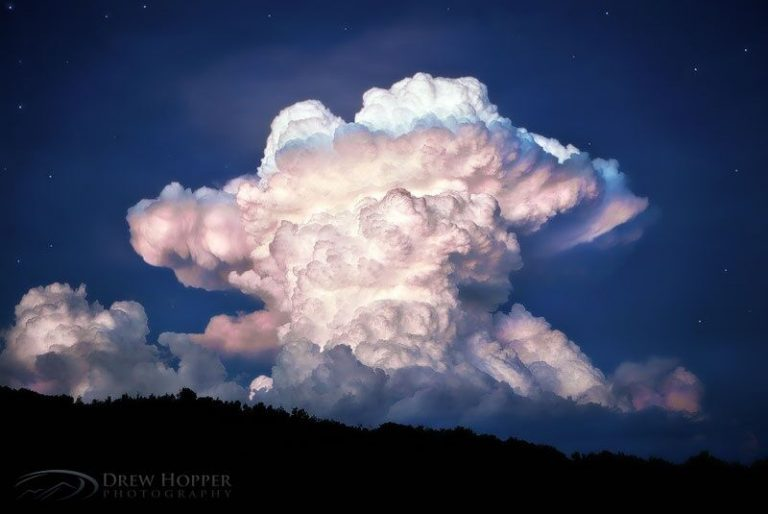
\includegraphics[width=0.95\textwidth]{figs/Fig-convectionCloud-HWeller-Pic-1-768x514.jpeg}
        \credit{Photo from H. Weller}{5pt}
    \end{column}
\end{columns}
        
\end{frame}

% GEOSTROPHIC APPROXIMATION %%%%%%%%%%%%%%%%%%%%%%%%%%%%%%%

\begin{frame}[t]{Atmospheric and ocean dynamics}

\vspace{-1.0em}

\begin{center}
\textbf{{\large
Atmospheric scale analysis for mid-latitude synoptic systems
}}
\end{center}

\small 
\center 

\vspace{-0.5em}

Horizontal equations

\begin{align*}
    &\textcolor{red}{    \frac{Du}{Dt}   }&
    &\textcolor{cyan}{   - \frac{uv \tan\phi}{a} + \frac{uw}{a}  }& 
    & \textcolor{blue}{   - 2\Omega v \sin\phi }
     \textcolor{blue}{  \,+ 2\Omega w \cos\phi }&
    & = &
    &\textcolor{teal}{   -\frac{1}{\rho}\frac{\partial p}{\partial x}  }&
    & \textcolor{purple}{\quad + \nu \nabla^2 u }&
    \\
    &\textcolor{red}{    \frac{Dv}{Dt}   } &
    &\textcolor{cyan}{   + \frac{u^2 \tan\phi}{a} + \frac{vw}{a}     }&
    & \textcolor{blue}{   + 2\Omega u \sin\phi    }&
    & = &
    &\textcolor{teal}{   -\frac{1}{\rho}\frac{\partial p}{\partial y}  }&
    & \textcolor{purple}{\quad + \nu \nabla^2 v }&
    \\ \\
      &\textcolor{black}{ \frac{U^2}{L}  }&
      &\textcolor{black}{ \quad \frac{UW}{a} \,\,\,\quad\quad\frac{U^2}{a} }&
      &\textcolor{black}{ \quad\quad f_0 U      }
       \textcolor{black}{\quad\quad\quad f_0 W  }&
      &&
      &\textcolor{black}{ \,\,\,\,\,\frac{\Delta P}{\rho L}  }&
      &\textcolor{black}{ \quad\frac{\nu U}{H^2} }&
    \\ \\
      &\textcolor{black}{ 10^{-4} }&
      &\textcolor{black}{ \quad10^{-5} \quad\quad\quad 10^{-8}  }&
      &\textcolor{black}{ \quad\quad10^{-3}        }
       \textcolor{black}{ \quad\quad\quad 10^{-6} }&
      &&
      &\textcolor{black}{ \quad10^{-3}  }&
      &\textcolor{black}{ \quad10^{-12} }&
\end{align*}

\end{frame}

\begin{frame}[t]{Atmospheric and ocean dynamics}

\vspace{-1.0em}

\begin{center}
\textbf{{\large
Atmospheric scale analysis for mid-latitude synoptic systems
}}
\end{center}

\small 
\center 

\vspace{-0.5em}

Horizontal equations

\begin{align*}
    &\textcolorg{red}{    \frac{Du}{Dt}   }&
    &\textcolorg{cyan}{   - \frac{uv \tan\phi}{a} + \frac{uw}{a}  }& 
    & \textcolor{blue}{   - 2\Omega v \sin\phi }
     \textcolorg{blue}{  \,+ 2\Omega w \cos\phi }&
    & = &
    &\textcolor{teal}{   -\frac{1}{\rho}\frac{\partial p}{\partial x}  }&
    & \textcolorg{purple}{\quad + \nu \nabla^2 u }&
    \\
    &\textcolorg{red}{    \frac{Dv}{Dt}   } &
    &\textcolorg{cyan}{   + \frac{u^2 \tan\phi}{a} + \frac{vw}{a}     }&
    & \textcolor{blue}{   + 2\Omega u \sin\phi    }&
    & = &
    &\textcolor{teal}{   -\frac{1}{\rho}\frac{\partial p}{\partial y}  }&
    & \textcolorg{purple}{\quad + \nu \nabla^2 v }&
    \\ \\
      &\textcolorg{black}{ \frac{U^2}{L}  }&
      &\textcolorg{black}{ \quad \frac{UW}{a} \,\,\,\quad\quad\frac{U^2}{a} }&
      &\textcolor{black}{ \quad\quad f_0 U      }
       \textcolorg{black}{\quad\quad\quad f_0 W  }&
      &&
      &\textcolor{black}{ \,\,\,\,\,\frac{\Delta P}{\rho L}  }&
      &\textcolorg{black}{ \quad\frac{\nu U}{H^2} }&
    \\ \\
      &\textcolorg{black}{ 10^{-4} }&
      &\textcolorg{black}{ \quad10^{-5} \quad\quad\quad 10^{-8}  }&
      &\textcolor{black}{ \quad\quad10^{-3}        }
       \textcolorg{black}{ \quad\quad\quad 10^{-6} }&
      &&
      &\textcolor{black}{ \quad10^{-3}  }&
      &\textcolorg{black}{ \quad10^{-12} }&
\end{align*}

\end{frame}

\begin{frame}[t]{Atmospheric and ocean dynamics}

\vspace{-1.0em}

\begin{center}
\textbf{{\large
Geostrophic approximation
}}
\end{center}

\small 
\center 

\vspace{-0.5em}

Horizontal equations

\vspace{-0.5em}

\normalsize

\begin{align*}
    \frac{1}{\rho}\frac{\partial p}{\partial x}
    -2\Omega v \sin\phi
    = 0
    \\
    \frac{1}{\rho}\frac{\partial p}{\partial y}
    +2\Omega u \sin\phi
    = 0
\end{align*}

\vspace{0.5em}

\begin{minipage}{0.8\textwidth}
\begin{flushleft}
    For large-scale mid-latitudinal flows there is an
intrinsic balance between the \textbf{pressure gradient force} and \textbf{Coriolis
force}. This is known as the \boldblue{geostrophic balance} and it leads to
air parcels traveling along lines of constant pressure.
\end{flushleft}
\end{minipage}

\end{frame}

\begin{frame}[t]{Atmospheric and ocean dynamics}

\vspace{-1.0em}

\begin{center}
\textbf{{\large
Geostrophic approximation
}}
\end{center}

\small 
\center 

\begin{minipage}{0.6\textwidth}
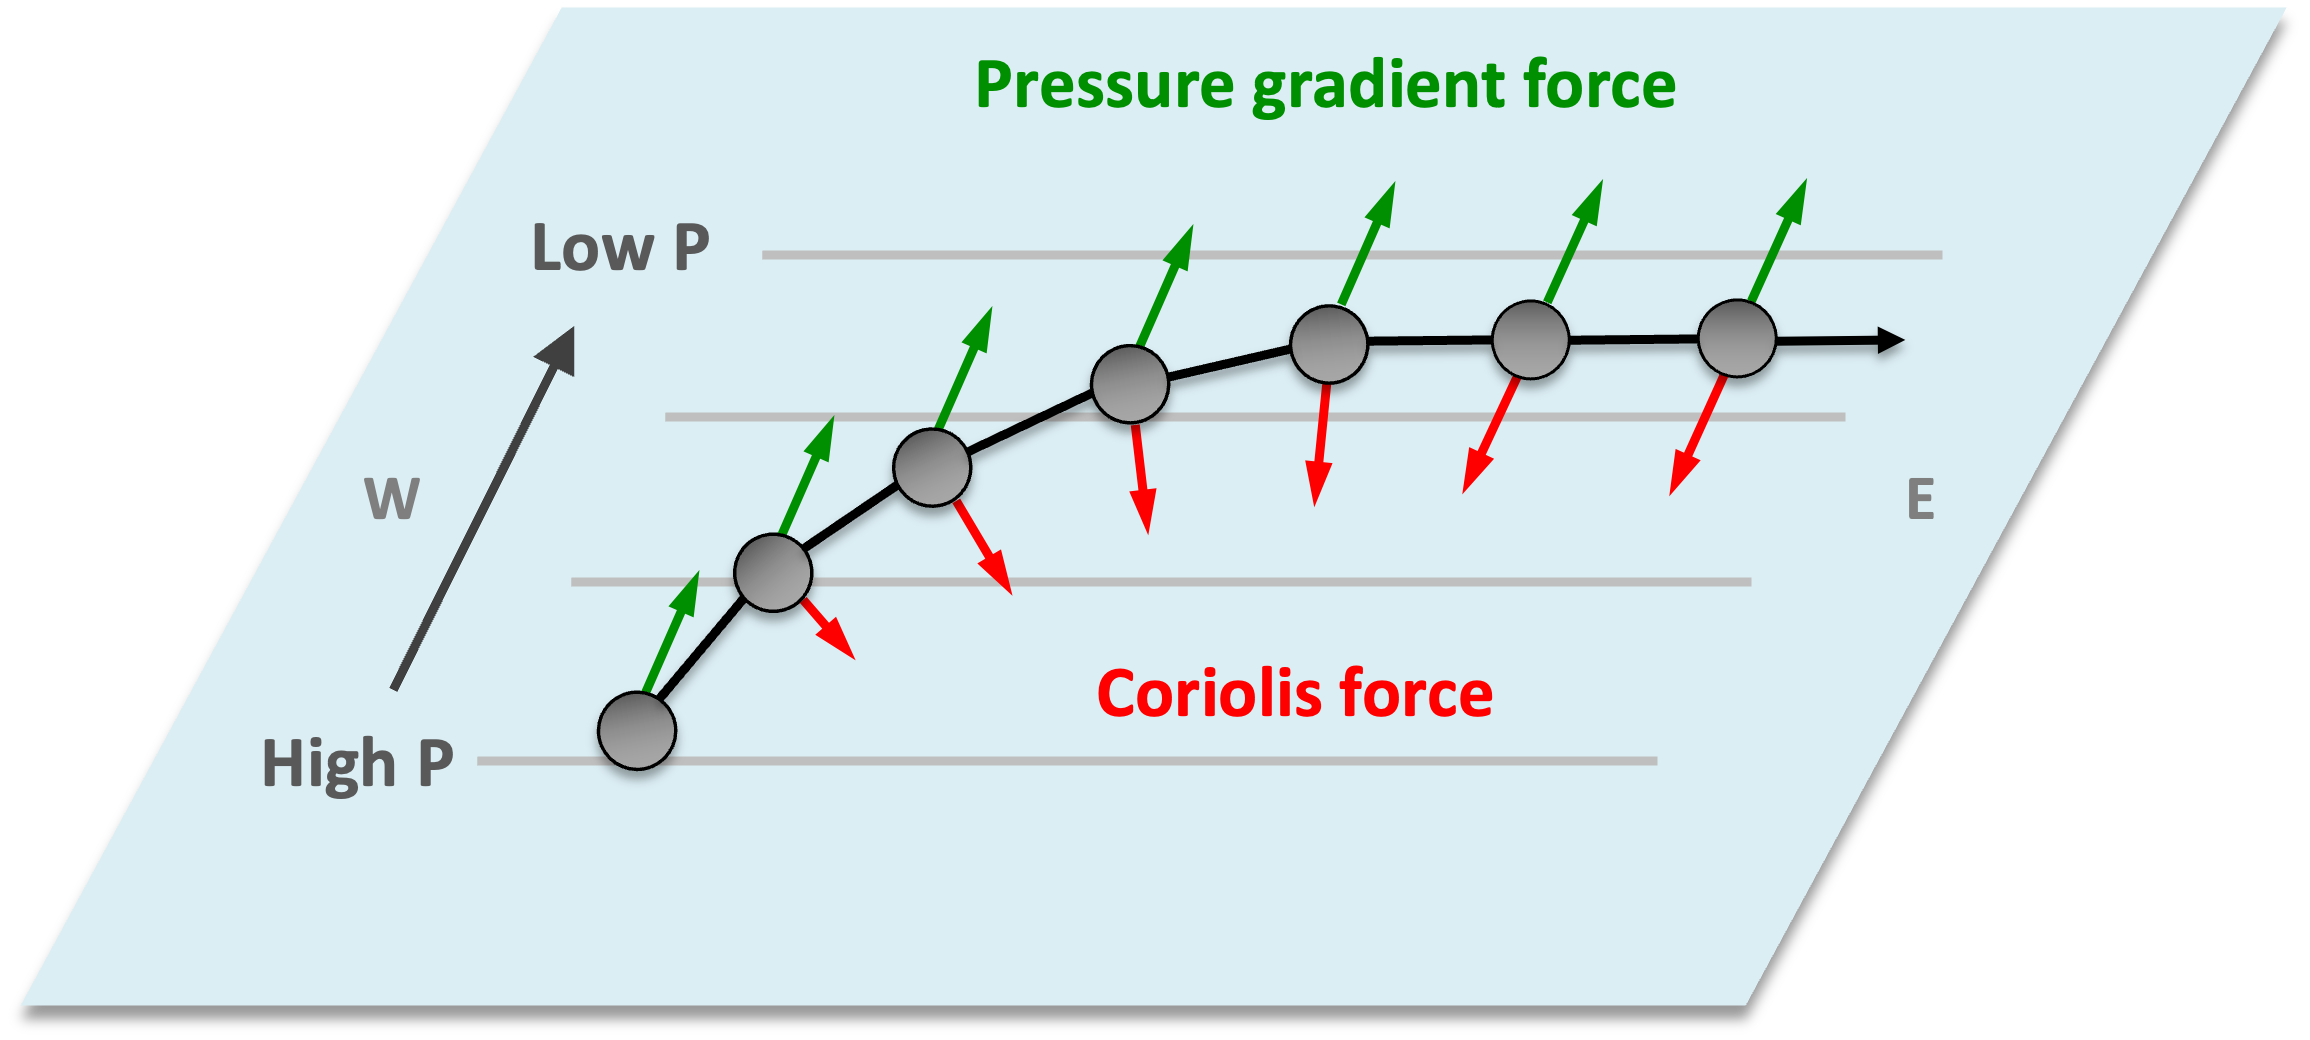
\includegraphics[width=0.9\textwidth]{figs/Fig-geostrophic-balance-ajr.png}
\end{minipage}

\vspace{1em}

\begin{minipage}{0.8\textwidth}
\begin{flushleft}
The geostrophic wind is the natural response of mid-latitudinal atmospheric motions to pressure gradients. It propagates perpendicular to the direction of the pressure gradient force and the Coriolis force (towards the East in the Northern and Southern hemispheres).
% Ullrich, Atmospheric Dyanmics, Lecture 6
\end{flushleft}
\end{minipage}

\end{frame}

\begin{frame}[t]{Atmospheric and ocean dynamics}

\vspace{-1.0em}

\begin{center}
\textbf{{\large
Geostrophic wind
% 500 Mb height contours together with wind speed vectors
}}
\end{center}

\small 
\center

\begin{minipage}{0.6\textwidth}
\begin{center}

{\color{darkgray}\scriptsize
1994-01-18 07:00
} \\[0.2em]
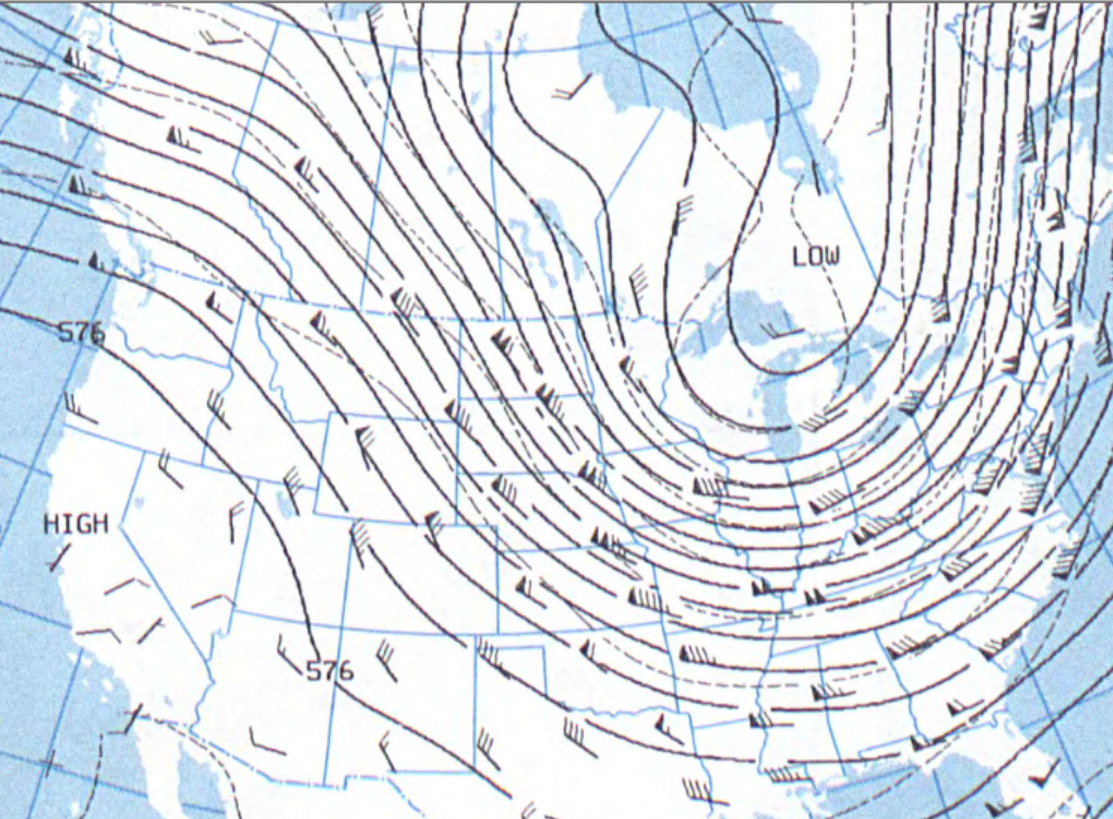
\includegraphics[width=0.9\textwidth]{figs/Fig-geostrophic-wind-NOAA-1994-01-18-07-00-500_Mb_Height_Contours.png}
\credit{NOAA}{5pt}

\end{center}
\end{minipage}

\end{frame}

%% OCEAN %%
\begin{frame}[t]{Ocean dynamics}
       
\small  

\vspace{-1.5em}

%Ullrich - Climate Lecture 8

\begin{columns}
    \begin{column}[t]{0.5\textwidth}
        \begin{center}
        \textbf{{\large
        Incompressibility
        }}
        \end{center}

        Seawater is \emph{nearly} incompressible. This means the mass conservation equation can be reduced to:
        \begin{align*}
            \nabla \cdot \mathbf{u} = 0
        \end{align*}

        \vspace{1em}
        
        \begin{center}
            \textbf{{\large
            Seawater density
            }}
        \end{center}
        
        The density of seawater is a function of temperature, salinity and pressure $\rho = \rho(T, S, p)$.

        In most cases, the dependence on pressure can be ignored, leaving $\rho = \rho(T, S)$.
        
    \end{column}
    \begin{column}[t]{0.5\textwidth}

        \begin{center}
        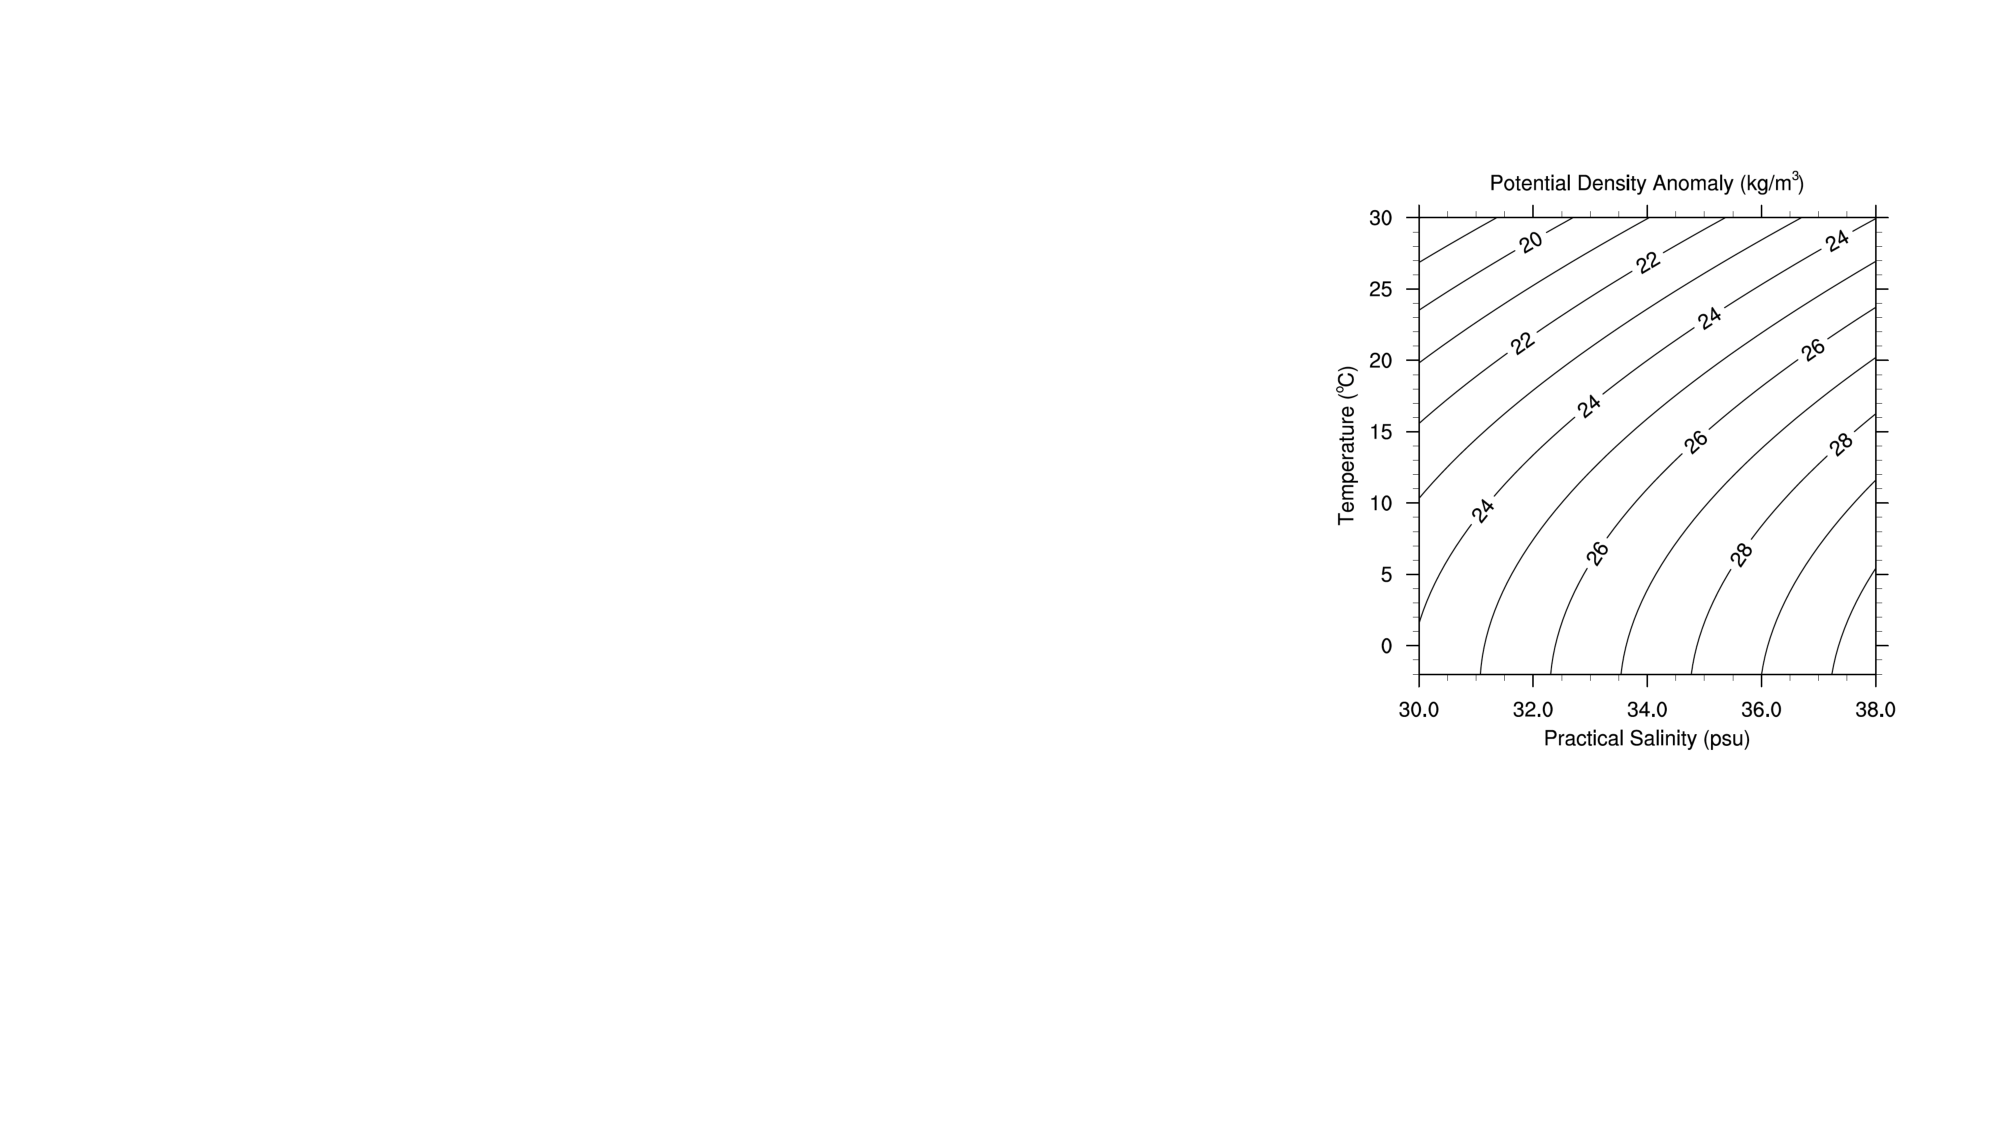
\includegraphics[width=0.8\textwidth]{figs/Fig-density-anomalies-Ullrich2020.pdf}
        \credit{Ullrich, 2020}{15pt}
        \end{center}
        
    \end{column}
\end{columns}
        
\end{frame}

% Hydrostatic Boussinesq approximation %%%%%%%%%%%%%%%%%

\begin{frame}[t]{Ocean dynamics}

\vspace{-1.0em}

\begin{center}
\textbf{{\large
Boussinesq approximation
}}
\end{center}

\small 
\center 

\vspace{-0.5em}

\begin{columns}
    \begin{column}{0.5\textwidth}
        \begin{flushleft}
            
            The \boldblue{Boussinesq approximation} assumes that density variations are negligible except where they appear in the buoyancy (gravity) term of the momentum equation.
            
            It is valid when:
            \begin{itemize}
                \item When density variations are small, typically less than a few percent.
                \item Vertical length scales ($H$) are much smaller than the density scale height.
            \end{itemize}
        
        \end{flushleft}
    \end{column}
    \begin{column}{0.5\textwidth}
        % fig from: https://rwu.pressbooks.pub/webboceanography/chapter/6-3-density/
        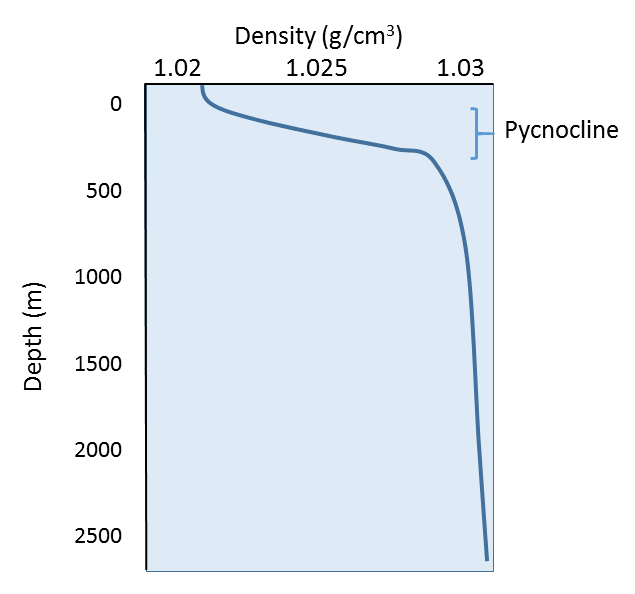
\includegraphics[width=0.9\textwidth]{figs/Fig-ocean-density-column-figure6.3.2.png}
        \credit{Webb, 2023}{40px}
    \end{column}
\end{columns}
        
\end{frame}

\begin{frame}[t]{Ocean dynamics}

\vspace{-0.5em}

\begin{center}
\textbf{{\large
Hydrostatic Boussinesq approximation
}}
\end{center}

\small 
\center 

\vspace{0em}

Incompressible flow that is in \textbf{hydrostatic balance}, \\
where density variations assumed to only affect buoyancy.

\begin{align*}
\text{Horizontal momentum:} \quad &
\frac{Du}{D t}
- f v
= -\frac{1}{\rho_0} \pdv{p}{x} + \mathcal{F}_u \\
%
 \quad &
\frac{Dv}{D t}
+ f u
= -\frac{1}{\rho_0} \pdv{p}{y} + \mathcal{F}_v \\[0.5em]
%
\text{Vertical momentum:} \quad &
\frac{1}{\rho_0}\pdv{p'}{z} = -g\frac{\rho'}{\rho_0} \textcolor{gray}{\quad\left[=b \right]} \\[0.5em]
%
\text{Continuity:} \quad &
\nabla \cdot \mathbf{u} = 0
\end{align*}

\vspace{-2em}

\begin{flushright}
\begin{minipage}{0.18\textwidth}
\begin{block}{}
    \footnotesize
    $\rho = \rho_0 + \rho',$ \\[0.5em]
    $\rho_0=1000\,\text{kg}\,\text{m}^{-3}$
\end{block}
\end{minipage}
\end{flushright}

\end{frame}

\begin{frame}[t]{Ocean dynamics}
\begin{center}

\vspace{-1.0em}

\textbf{{\large
Hydrostatic Boussinesq approximation
}}

\vspace{2.0em}

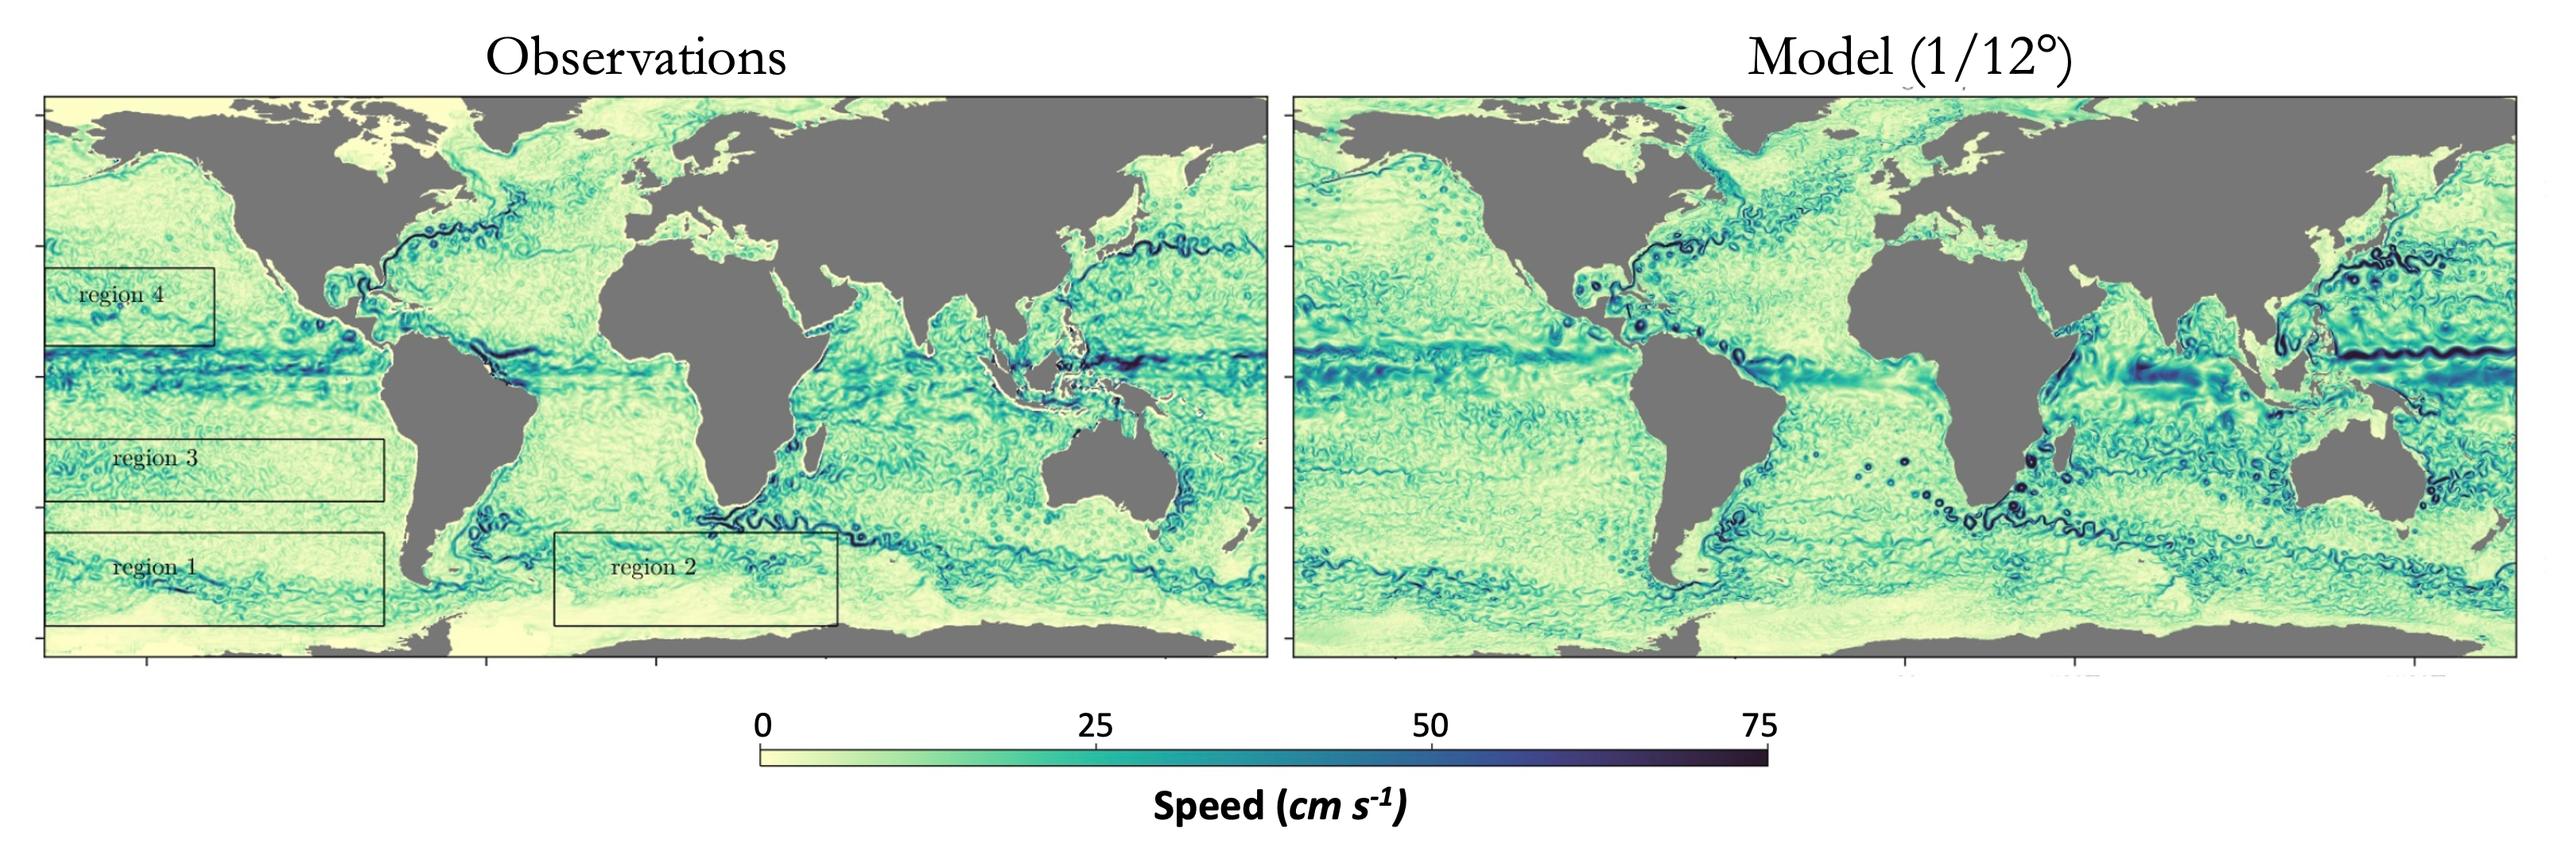
\includegraphics[width=0.95\textwidth]{figs/Fig-oceananigans-Silvestri2025-2.png}
\credit{Silvestri et al., 2025}{15pt}

\end{center}
\end{frame}

%% Ice sheets %%

\begin{frame}{}

\centering

{\huge 
Ice-sheet dynamics
}

\end{frame}

\begin{frame}[t]{Ice-sheet dynamics}

\vspace{-0.5em}

\begin{columns}
    \begin{column}{0.5\textwidth}
        Ice-sheet dynamics are governed by viscous, non-Newtonian, gravitationally driven flow, called \boldblue{creeping flow} or \boldblue{Stokes flow}.
        \newline
        
        This type of flow is \text{very slow} and \text{very viscous}, so the Reynolds number is \textbf{very small}:
        \begin{align*}
            \text{Re}= \frac{UL}{\nu} \ll 1
        \end{align*}

        \begin{block}{}
            {\footnotesize
            Recall that in \textbf{Non-Newtonian flow}, there is a non-linear relationship between stress and strain.
            }
        \end{block}
        
    \end{column}
    \begin{column}{0.5\textwidth}
        \centering
        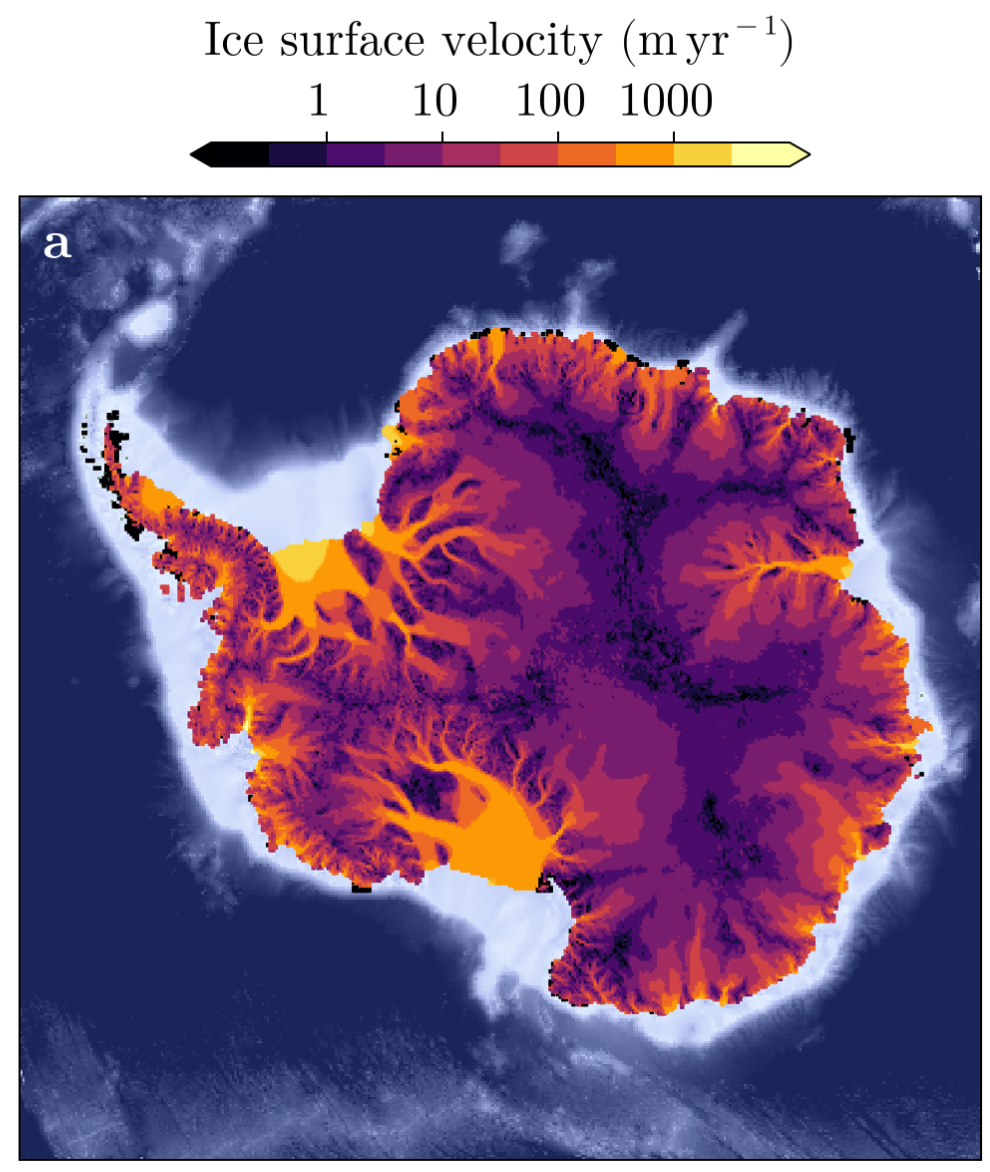
\includegraphics[width=0.85\textwidth]{figs/Fig-Antarctica-surface-velocity.png}
        %\begin{flushright}
        %{\color{lightgray} {\small J. Swierczek-Jereczek}}
        %\end{flushright}
    \end{column}
\end{columns}
\centering
        
\end{frame}

\begin{frame}[t]{Ice-sheet dynamics}

\vspace{-1.0em}

\begin{center}
\textbf{{\large
Incompressible Non-Newtonian Stokes Equation
}}
\end{center}

\small 
\center 

\vspace{-0.5em}

\begin{align*}
&\text{Momentum (no inertia):} \quad 
0 = -\nabla p + \nabla \cdot \boldsymbol{\tau} - \rho \mathbf{g} \\
&\text{Mass conservation:} \quad\quad\quad\, 
 \nabla \cdot \mathbf{u} = 0
\end{align*}
\newline
% \begin{align*}
% &\text{Constitutive law (non-Newtonian):} && 
% \boldsymbol{\tau} = 2 \eta(\dot{\varepsilon}) \, \mathbf{D} \\
% &\text{Strain-rate tensor:} && 
% \mathbf{D} = \frac{1}{2} \left( \nabla \mathbf{u} + \nabla \mathbf{u}^T \right) \\
% &\text{Viscosity (Glen's flow law):} &&
% \eta = \frac{1}{2} A^{-1/n} \dot{\varepsilon}_e^{(1-n)/n}, \quad A = f(T)
% \end{align*}

\end{frame}

\begin{frame}[t]{Ice-sheet dynamics}

\vspace{-1.0em}

\begin{center}
\textbf{{\large
Incompressible Non-Newtonian Stokes Equation
}}
\end{center}

\small 
\center 

\vspace{-0.5em}

\begin{align*}
&\text{Momentum (no inertia):} \quad 
0 = -\nabla p \textcolor{Plum}{\,+\, \nabla \cdot \boldsymbol{\tau}} - \rho \mathbf{g} \\
&\text{Mass conservation:} \quad\quad\quad\, 
 \nabla \cdot \mathbf{u} = 0
\end{align*}
\newline
\begin{align*}
&\text{Constitutive law (non-Newtonian):} && 
\boldsymbol{\tau} = 2 \eta(\dot{\varepsilon}) \, \mathbf{D} \\
&\text{Strain-rate tensor:} && 
\mathbf{D} = \frac{1}{2} \left( \nabla \mathbf{u} + \nabla \mathbf{u}^T \right) \\
&\text{Viscosity (Glen's flow law):} &&
\eta = \frac{1}{2} A^{-1/n} \dot{\varepsilon}_e^{(1-n)/n}, \quad A = f(T)
\end{align*}

\end{frame}

\begin{frame}[t]{Ice-sheet dynamics}

\vspace{-1.0em}

\begin{center}
\textbf{{\large
Incompressible Non-Newtonian Stokes Equation
}}
\end{center}

\small 
\center 

\vspace{-0.5em}

\begin{align*}
&\text{Momentum (no inertia):} \quad 
\nabla \cdot \boldsymbol{\tau} = \nabla p  + \rho \mathbf{g} \\
&\text{Mass conservation:} \quad\quad\quad\, 
 \nabla \cdot \mathbf{u} = 0
\end{align*}
\newline
\begin{align*}
&\text{Constitutive law (non-Newtonian):} && 
\boldsymbol{\tau} = 2 \eta(\dot{\varepsilon}) \, \mathbf{D} \\
&\text{Strain-rate tensor:} && 
\mathbf{D} = \frac{1}{2} \left( \nabla \mathbf{u} + \nabla \mathbf{u}^T \right) \\
&\text{Viscosity (Glen's flow law):} &&
\eta = \frac{1}{2} A^{-1/n} \dot{\varepsilon}_e^{(1-n)/n}, \quad A = f(T)
\end{align*}

\end{frame}

\begin{frame}[t]{Ice-sheet dynamics}

\vspace{-1.0em}

\begin{center}
\textbf{{\large
Incompressible Non-Newtonian Stokes Equation
}}
\end{center}

\footnotesize 
\centering

\vspace{-0.5em}

\begin{align*}
&\text{Momentum:} &&\\
&\quad\quad\quad
\textcolor{Plum}{
\pdv{}{x} \left( 2\eta \pdv{u}{x} \right)
+ \pdv{}{y} \left( \eta \left( \pdv{u}{y} + \pdv{v}{x} \right) \right)
+ \pdv{}{z} \left( \eta \left( \pdv{u}{z} + \pdv{w}{x} \right) \right)
} 
&&=
\,\textcolor{teal}{   \pdv{p}{x} }
\\[0.5em]
&\quad\quad\quad
\textcolor{Plum}{
\pdv{}{x} \left( \eta \left( \pdv{u}{y} + \pdv{v}{x} \right) \right)
+ \pdv{}{y} \left( 2\eta \pdv{v}{y} \right)
+ \pdv{}{z} \left( \eta \left( \pdv{v}{z} + \pdv{w}{y} \right) \right)
}
&&=
\,\textcolor{teal}{   \pdv{p}{y} }
\\[0.5em]
&\quad\quad\quad
\textcolor{Plum}{
+ \pdv{}{x} \left( \eta \left( \pdv{u}{z} + \pdv{w}{x} \right) \right)
+ \pdv{}{y} \left( \eta \left( \pdv{v}{z} + \pdv{w}{y} \right) \right)
+ \pdv{}{z} \left( 2\eta \pdv{w}{z} \right) }  
&&=
\,\textcolor{teal}{   \pdv{p}{z} }
\textcolor{orange}{ + \rho g    }
\\[0.5em]
&\text{Mass conservation:} \quad 
 \nabla \cdot \mathbf{u} = 0 &&
\end{align*}

\begin{columns}
    \begin{column}{0.6\textwidth}
    \end{column}
    \begin{column}{0.4\textwidth}
        \begin{flushright}
            \vspace{-2em}
            %{\footnotesize 
            %\textcolor{teal}{Pressure gradient} \\
            %\textcolor{Plum}{Dissipation (internal stress)} \\
            %\textcolor{orange}{Gravity}
            %}
        \end{flushright}
    \end{column}
\end{columns}

\end{frame}

\begin{frame}[t]{Ice-sheet dynamics}

\vspace{-1.0em}

\begin{center}
\textbf{{\large
Blatter-Pattyn approximation
}}
\end{center}

\small 
\centering

\vspace{1.5em}

\begin{minipage}{0.8\textwidth}
{\flushleft

\begin{itemize}
    \item Apply the hydrostatic approximation in the vertical.
    \item Assumes horizontal gradients of the vertical velocity are small \\ compared to the vertical gradient of the horizontal velocity:  \\
    \vspace{0.3em}
    \hspace{70pt} $\pdv{w}{x} \ll \pdv{u}{z}$, $\quad$ $\pdv{w}{y} \ll \pdv{v}{z}$
    \item Assume a zero normal stress at the surface (stress-free condition).
\end{itemize}

\vspace{2.0em}

This eliminate pressure as a prognostic variable and reduces the problem to two equations (solving for $u$ and $v$) -- $w$ is diagnosed from mass conservation.

}
\end{minipage}

\end{frame}

\begin{frame}[t]{Ice-sheet dynamics}

\vspace{-1.0em}

\begin{center}
\textbf{{\large
Blatter-Pattyn approximation
}}
\end{center}

\small 
\center 

\vspace{-0.5em}
 
    \begin{align*}
    &\text{Momentum:}& \\
    &\quad\quad\quad 
    \pdv{}{x} \left( 4\eta \pdv{u}{x} + 2\eta \pdv{v}{y}\right) +
    \pdv{}{y} \left(  \eta \pdv{u}{y} + \eta \pdv{v}{x} \right) +
    \pdv{}{z} \left( \eta \pdv{u}{z} \right) \,\,\,= \,\rho g \pdv{s}{x} \\[0.5em]
    &\quad\quad\quad 
    \pdv{}{x} \left( \eta \pdv{u}{y} + \eta \pdv{v}{x} \right) + \pdv{}{y} \left( 4\eta \pdv{v}{y} + 2\eta \pdv{u}{x} \right) +
    \pdv{}{z} \left( \eta \pdv{v}{z} \right) = \,\rho g \pdv{s}{y} \\[1em]
    &\text{Continuity:} \quad
    \nabla \cdot \mathbf{u} = 0 &
    \end{align*}
\end{frame}

\begin{frame}[t]{Ice-sheet dynamics}

    \vspace{-1.0em}

    \begin{center}
    \textbf{{\large
    Shallow-shelf approximation (SSA)
    }}
    \end{center}
    
    \small 
    \center 
    
    \vspace{-0.5em}
     
    \begin{itemize}
        \item Hydrostatic approximation.
        \item Shallow approximation ($H \ll L$) $\rightarrow$ vertically integrated.
        \item Assumes gravitational driving stress is balanced by longitudinal stress.
    \end{itemize}

    \begin{align*}
        \text{Momentum:}& \quad 
        \pdv{}{x} \left( 4\bar{\eta}H\pdv{\bar{u}}{x} + 2\bar{\eta}H \pdv{\bar{v}}{y} \right) +
        \pdv{}{y} \left( \bar{\eta}H\pdv{\bar{u}}{y} + \bar{\eta}H\pdv{\bar{v}}{x} \right) =
        \rho g H \pdv{s}{x} \\[1em]
        & \quad
        \pdv{}{y} \left( 4\bar{\eta}H\pdv{\bar{v}}{y} + 2\bar{\eta}H\pdv{\bar{u}}{x} \right) +
        \pdv{}{x} \left( \bar{\eta}H\pdv{\bar{u}}{y} + \bar{\eta}H\pdv{\bar{v}}{x} \right)
        =
        \rho g H \pdv{s}{y} \\[0.5em]
        \text{Continuity:}& \quad
        \nabla \cdot \mathbf{u} = 0
    \end{align*}

\end{frame}

\begin{frame}[t]{Ice-sheet dynamics}

    \vspace{-1.0em}

    \begin{center}
    \textbf{{\large
    Shallow-ice approximation (SIA)
    }}
    \end{center}
    
    \small 
    \center 
    
    \vspace{-0.5em}
    
    \begin{itemize}
        \item Hydrostatic approximation.
        \item Shallow approximation ($H \ll L$) $\rightarrow$ vertically integrated (sometimes).
        \item Assumes gravitational driving stress is balanced by vertical shear stress.
    \end{itemize}

    \begin{align*}
        \text{Momentum:}& \quad 
        \pdv{}{z} \left( \eta \pdv{u}{z} \right) = \rho g \pdv{s}{x} \\[0.5em]
        & \quad
        \pdv{}{z} \left( \eta \pdv{v}{z} \right) = \rho g \pdv{s}{y} \\[1em]
        \text{Continuity:}& \quad
        \nabla \cdot \mathbf{u} = 0
    \end{align*}

\end{frame}

\begin{frame}{Ice-sheet dynamics}
\begin{center}

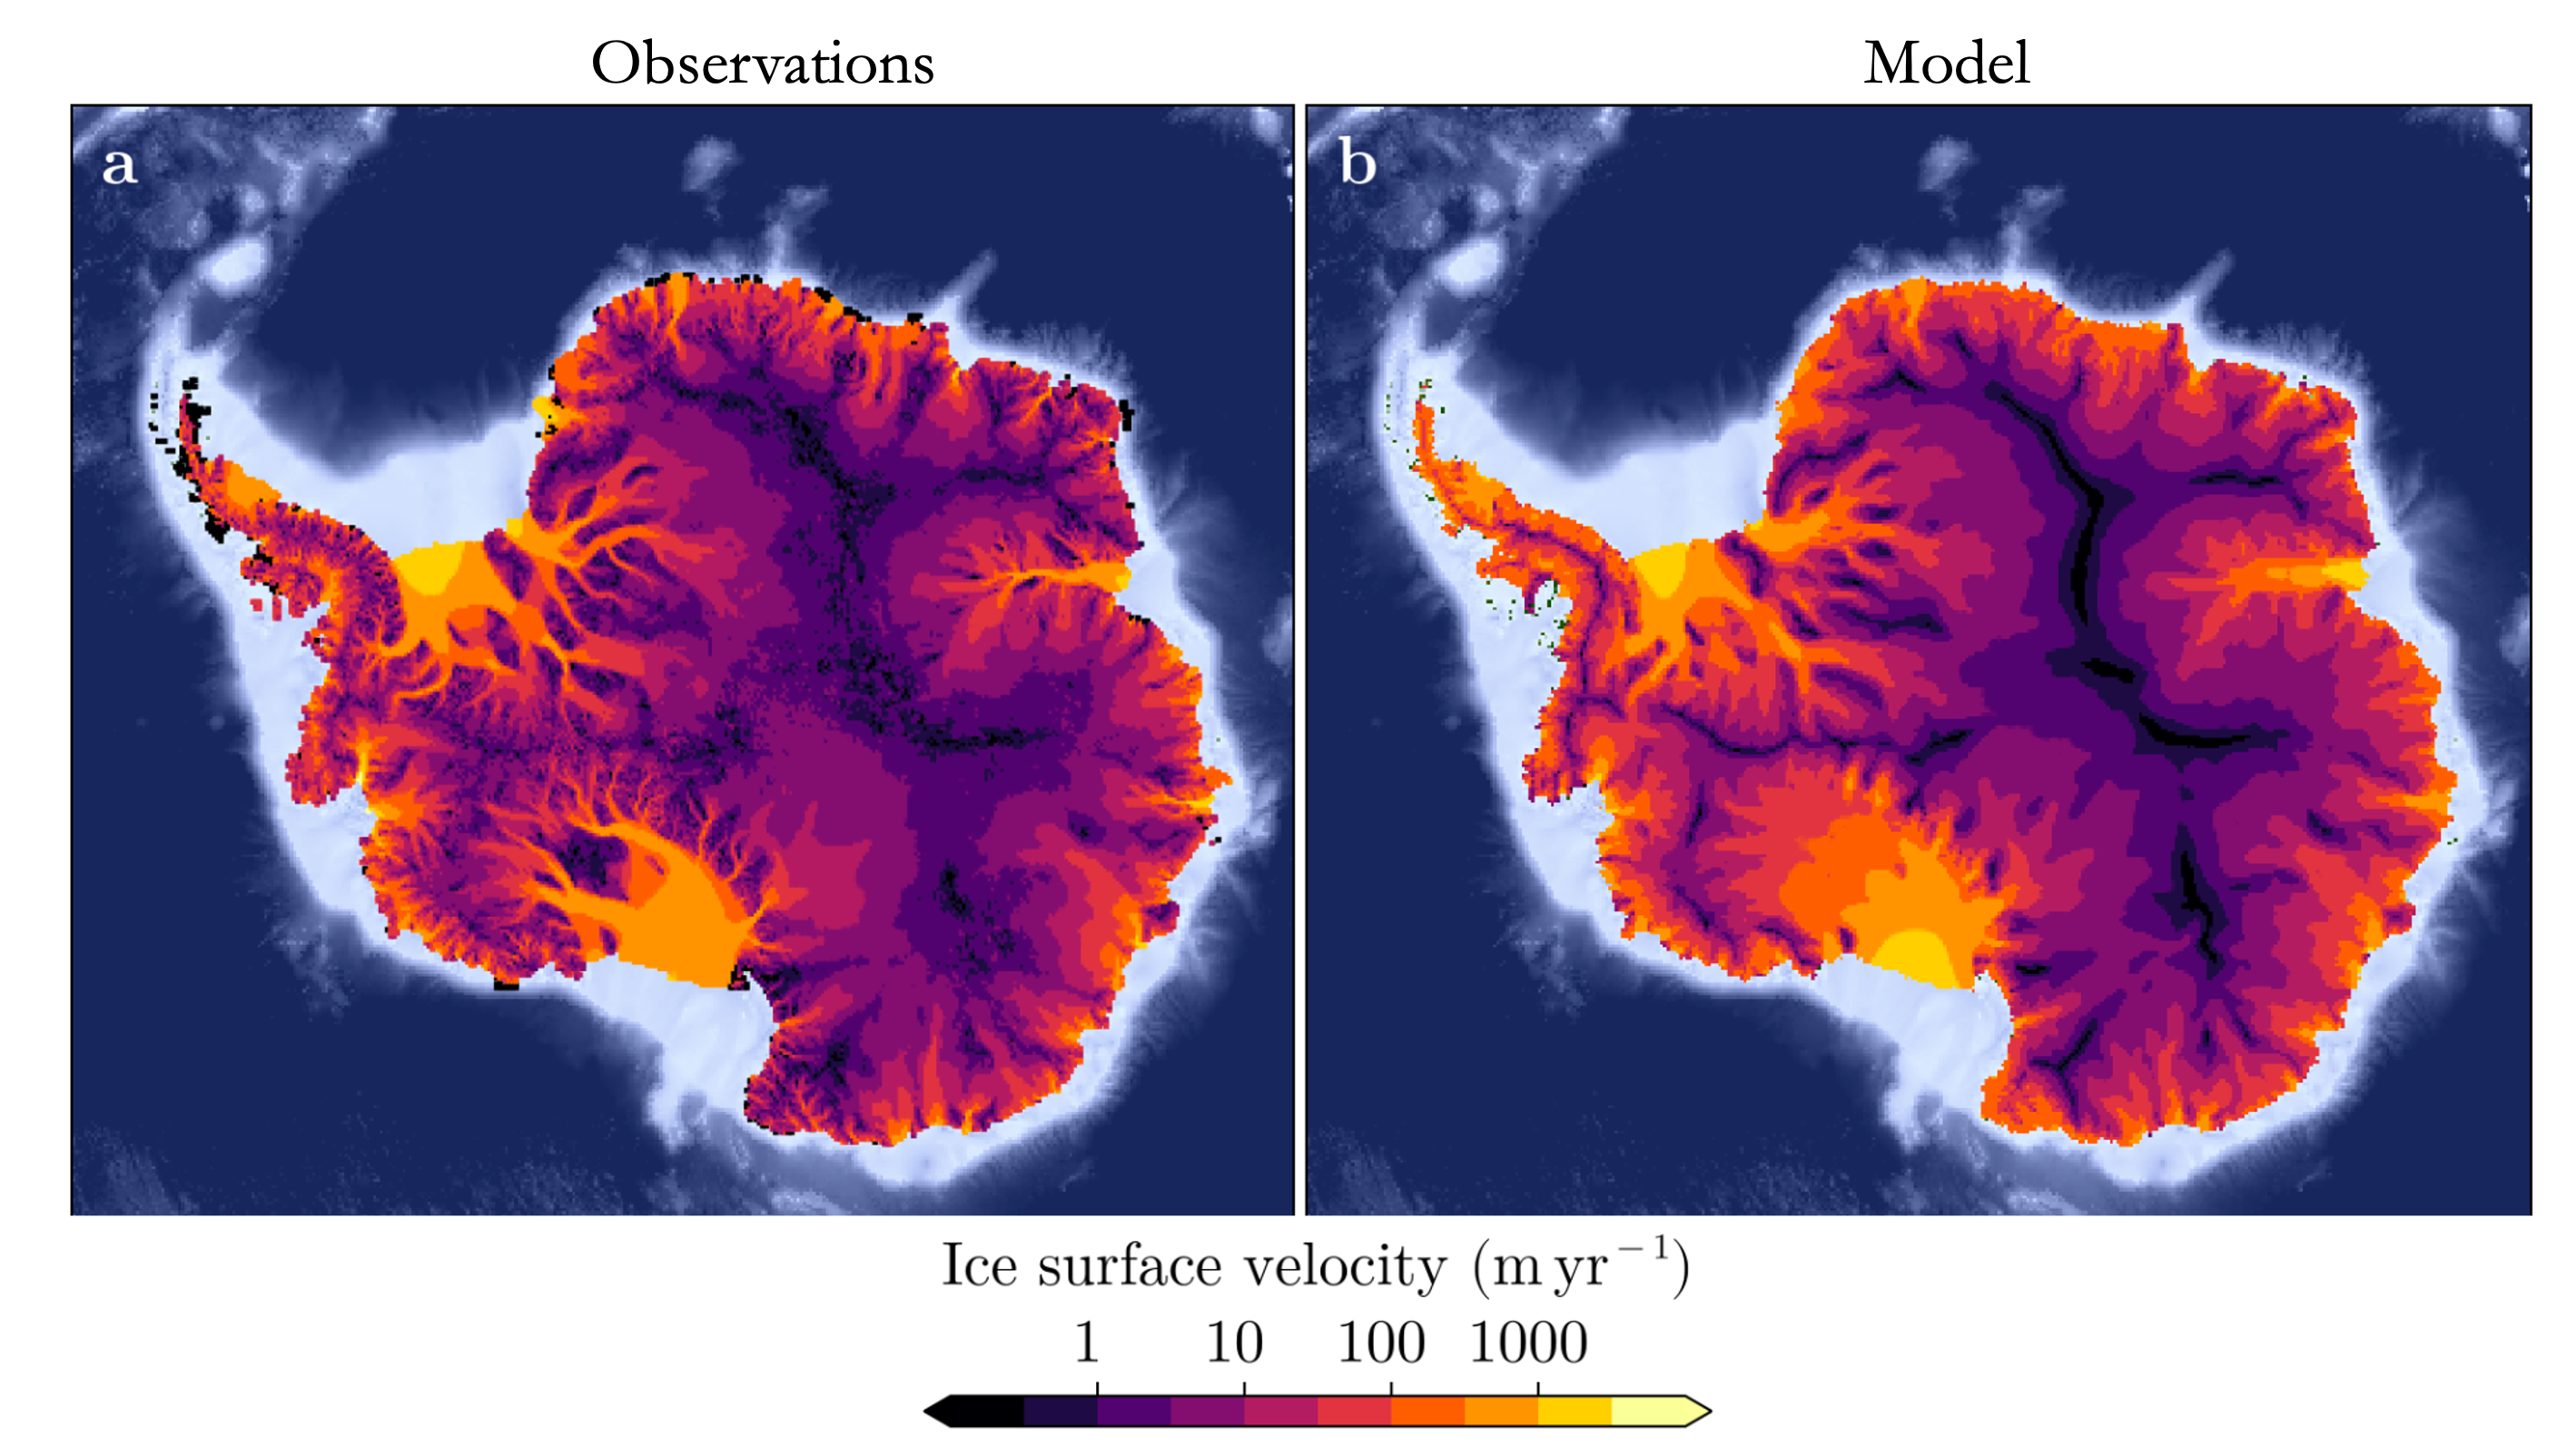
\includegraphics[width=0.8\textwidth]{figs/Fig-Antarctica-surface-velocity-with-model.png}
\credit{Swierczek-Jereczek et al.}{10pt}

\end{center}
\end{frame}


%%% SUMMARY %%%%

\begin{frame}{Geophysical fluid dynamics summary}

Relevant terms for each system

\begin{table}[h!]
\centering
\renewcommand{\arraystretch}{1.4}
\begin{tabular}{@{}lcccc@{}}
\toprule
\textbf{Term} & \textbf{Atmosphere} & \textbf{Ocean} & \textbf{Ice Sheets} \\ \midrule
Inertia              & X   & X   &     \\
Curvature            & X   & X   &     \\
Coriolis             & X   & X   &     \\
Pressure Gradient    & X   & X   & X\hspace{0.5em}   \\
Gravity              & X   & X   & X\hspace{0.5em}   \\
Friction/Dissipation & X   & X   & X\textbf{*}\\
\bottomrule
\end{tabular}
\end{table}
\hspace{25em}\textbf{*}Non-Newtonian fluid

\end{frame}

\begin{frame}{Summary of common approximations}

\vspace{1em}

\begin{columns}
    \begin{column}{0.15\textwidth}
    \end{column}
    \begin{column}{0.85\textwidth}
        \textbf{Atmosphere/ocean}
        \begin{itemize}
            \item Shallow atmosphere/ocean approximation
            \item Hydrostatic approximation
            \item Geostrophic approximation
            \item Boussinesq approximation (ocean)
        \end{itemize}

        \vspace{1em}
        
        \textbf{Ice sheets}
        \begin{itemize}
            \item Blatter-Pattyn approximation
            \item Shallow-shelf approximation
            \item Shallow-ice approximation
        \end{itemize}
    \end{column}
\end{columns}

\end{frame}

\begin{frame}{Useful references}

\begin{center}

% Holton 2004 %%%%%%%%%%%%%%%%%%%%%%%%%%%%%%%%%%%
\begin{minipage}{0.18\textwidth}
\begin{center}
\textbf{Holton, 2004}

\vspace{1em}

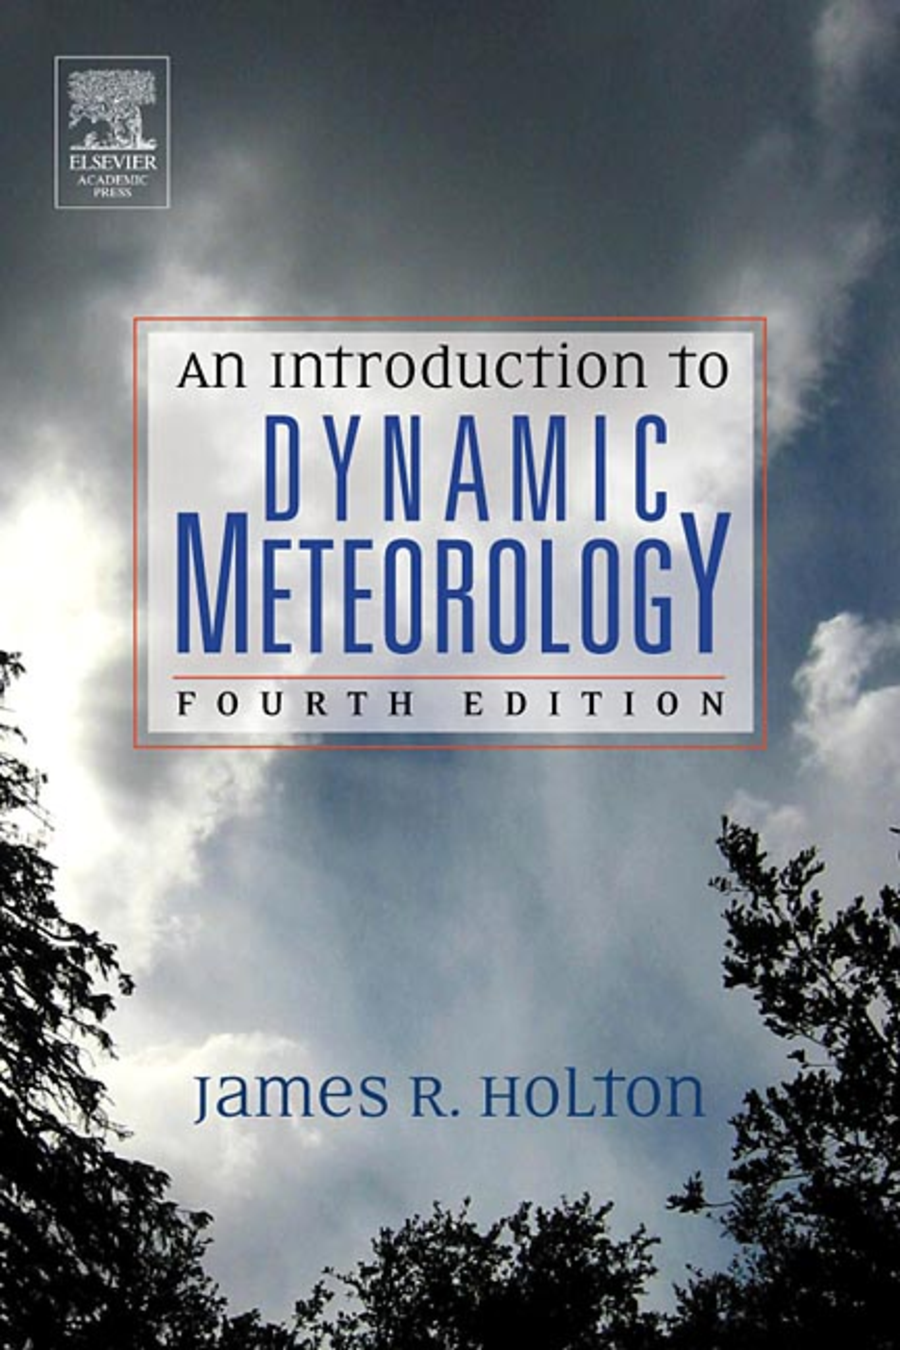
\includegraphics[width=1\textwidth]{figs/Fig-Book-Holton-2004.pdf}
\end{center}
\end{minipage}
\hspace{1em}
% Marshall and Plumb 2008 %%%%%%%%%%%%%%%%%%%%%%%%%%%%%%%%%%%
\begin{minipage}{0.18\textwidth}
\begin{center}
\textbf{Marshall and Plumb, 2008}

\vspace{1em}

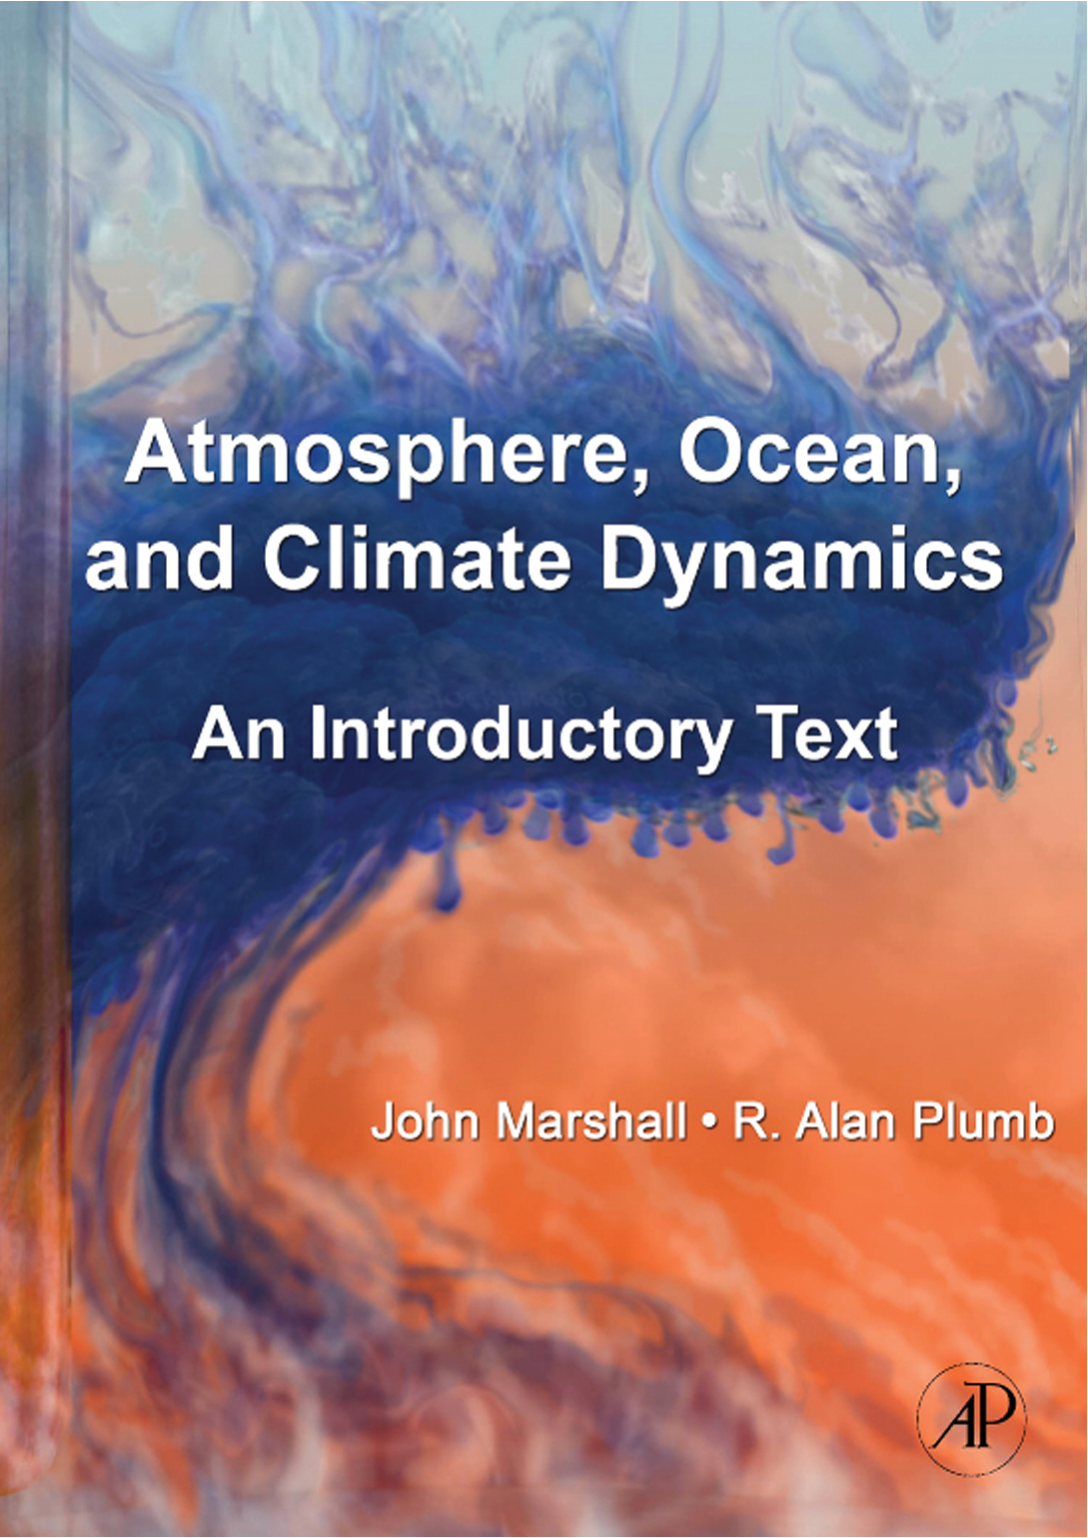
\includegraphics[width=1\textwidth]{figs/Fig-Book-Marshall-Plumb-2008.pdf}
\end{center}
\end{minipage}
\hspace{1em}
% Vallis, 2017 %%%%%%%%%%%%%%%%%%%%%%%%%%%%%%%%%%%
\begin{minipage}{0.2\textwidth}
\begin{center}
\textbf{Vallis, 2017}

\vspace{1em}

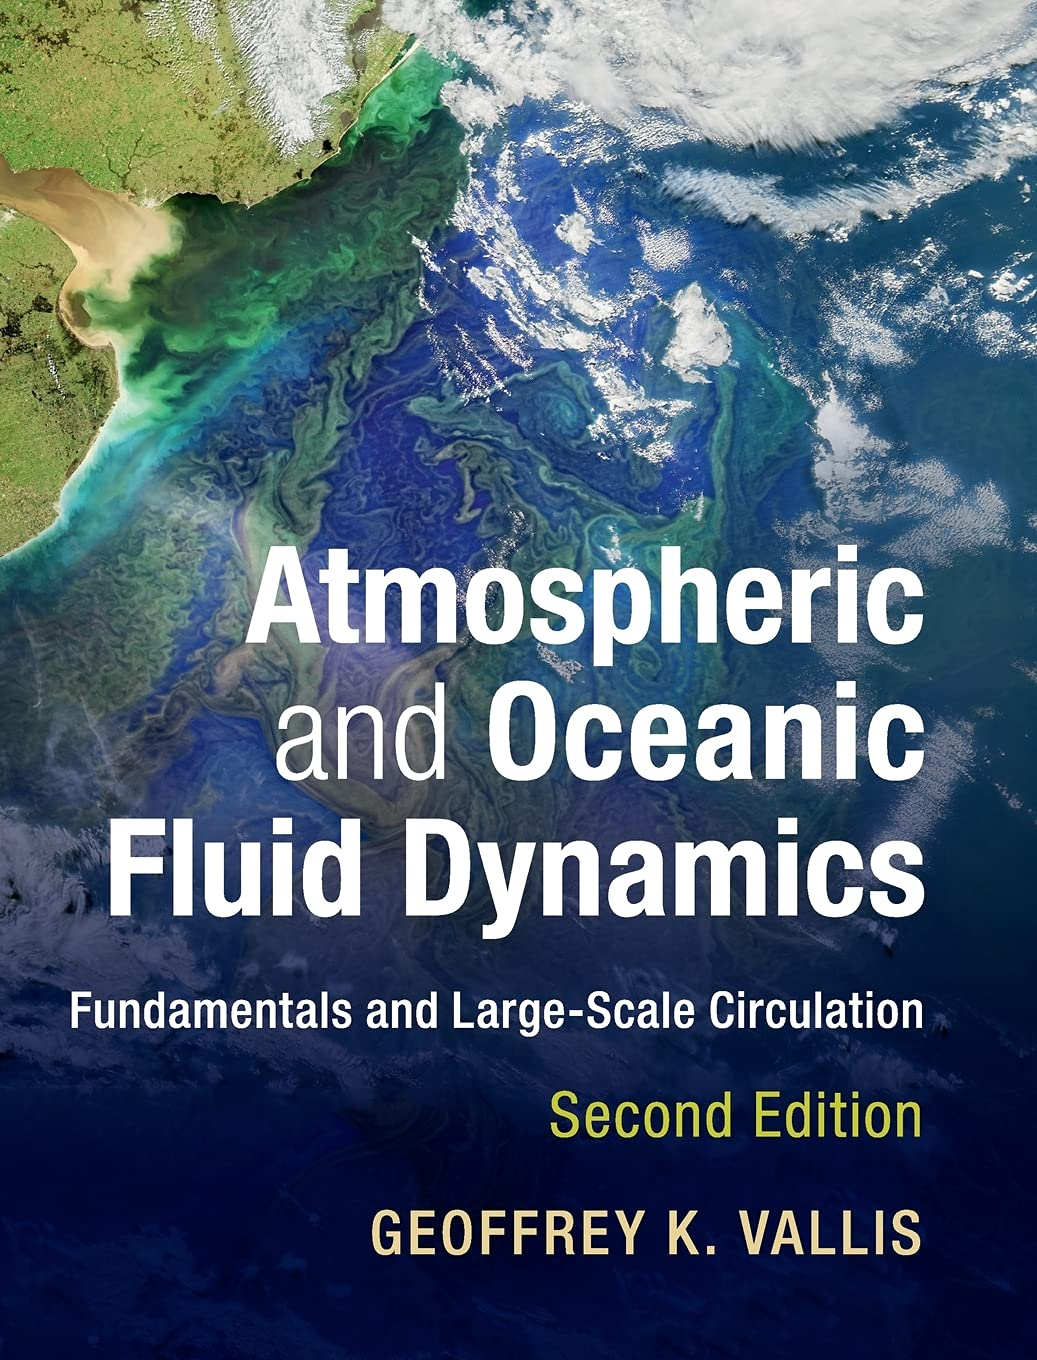
\includegraphics[width=1\textwidth]{figs/Fig-Book-Vallis-2017.jpg}
\end{center}
\end{minipage}
\hspace{1em}
% Greve and Blatter, 2009 %%%%%%%%%%%%%%%%%%%%%%%%%%%%%%%%%%%
\begin{minipage}{0.2\textwidth}
\begin{center}
\textbf{Greve and Blatter, 2009}

\vspace{1em}

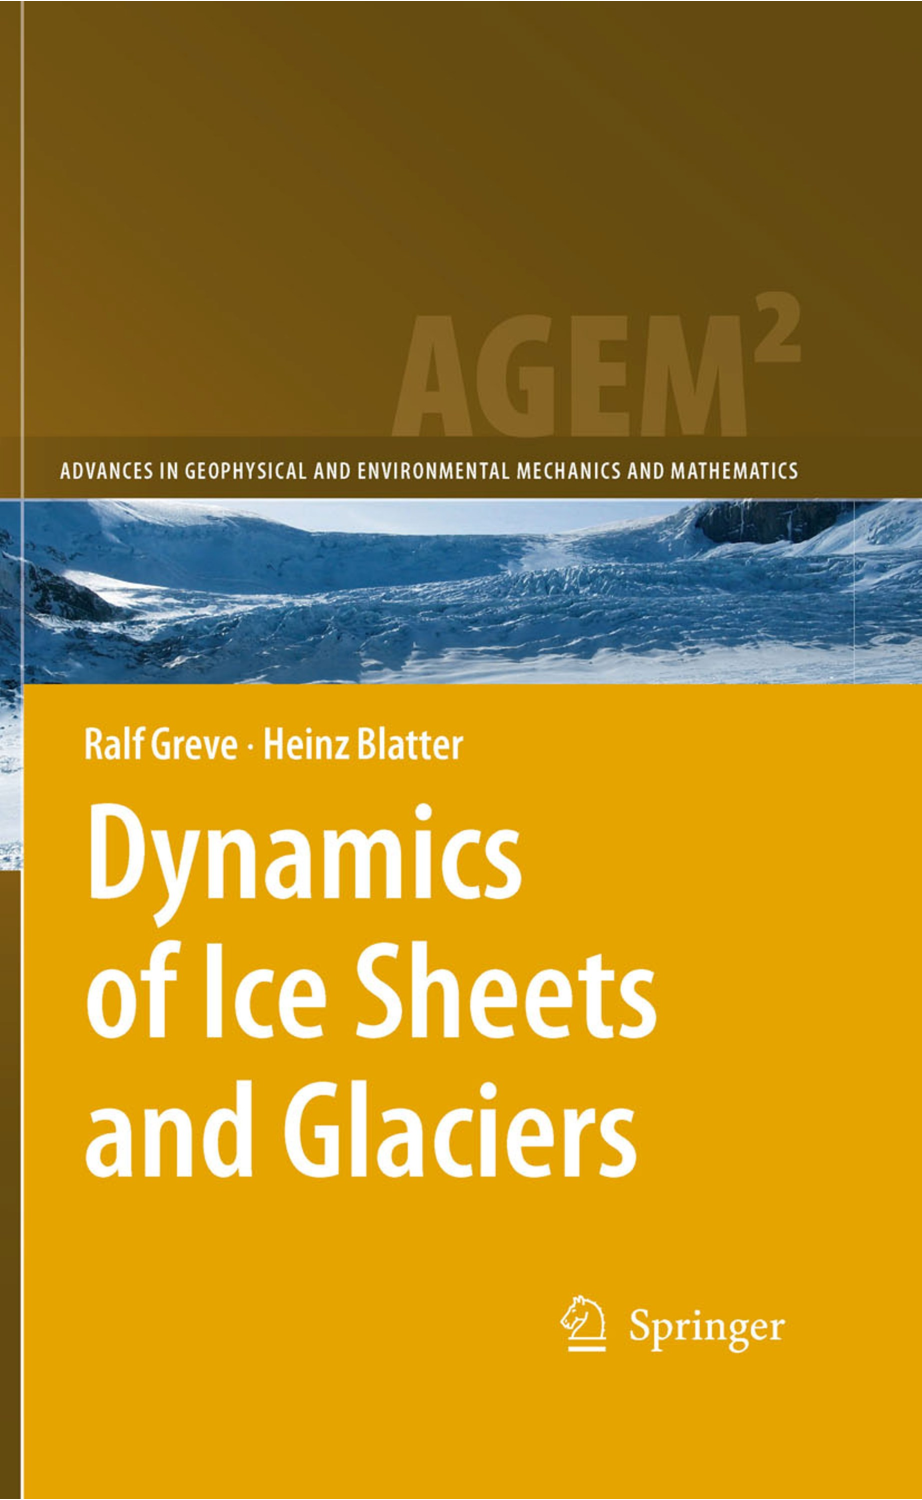
\includegraphics[width=0.8\textwidth]{figs/Fig-Book-Greve-Blatter-2009.pdf}
\end{center}
\end{minipage}

\end{center}

\end{frame}

\appendix

%% EMPTY SLIDE: END OF PRESENTATION %%
\begin{frame}
\end{frame}
%%%%%%%%%%%%%%%%%%%%%%%%%%%%%%%%%

%% BONUS SLIDES %%

% Something to transition to talking about scale analysis
\begin{frame}{Scale analysis: tropical cyclone}
\begin{columns}
    \begin{column}{0.5\textwidth}
        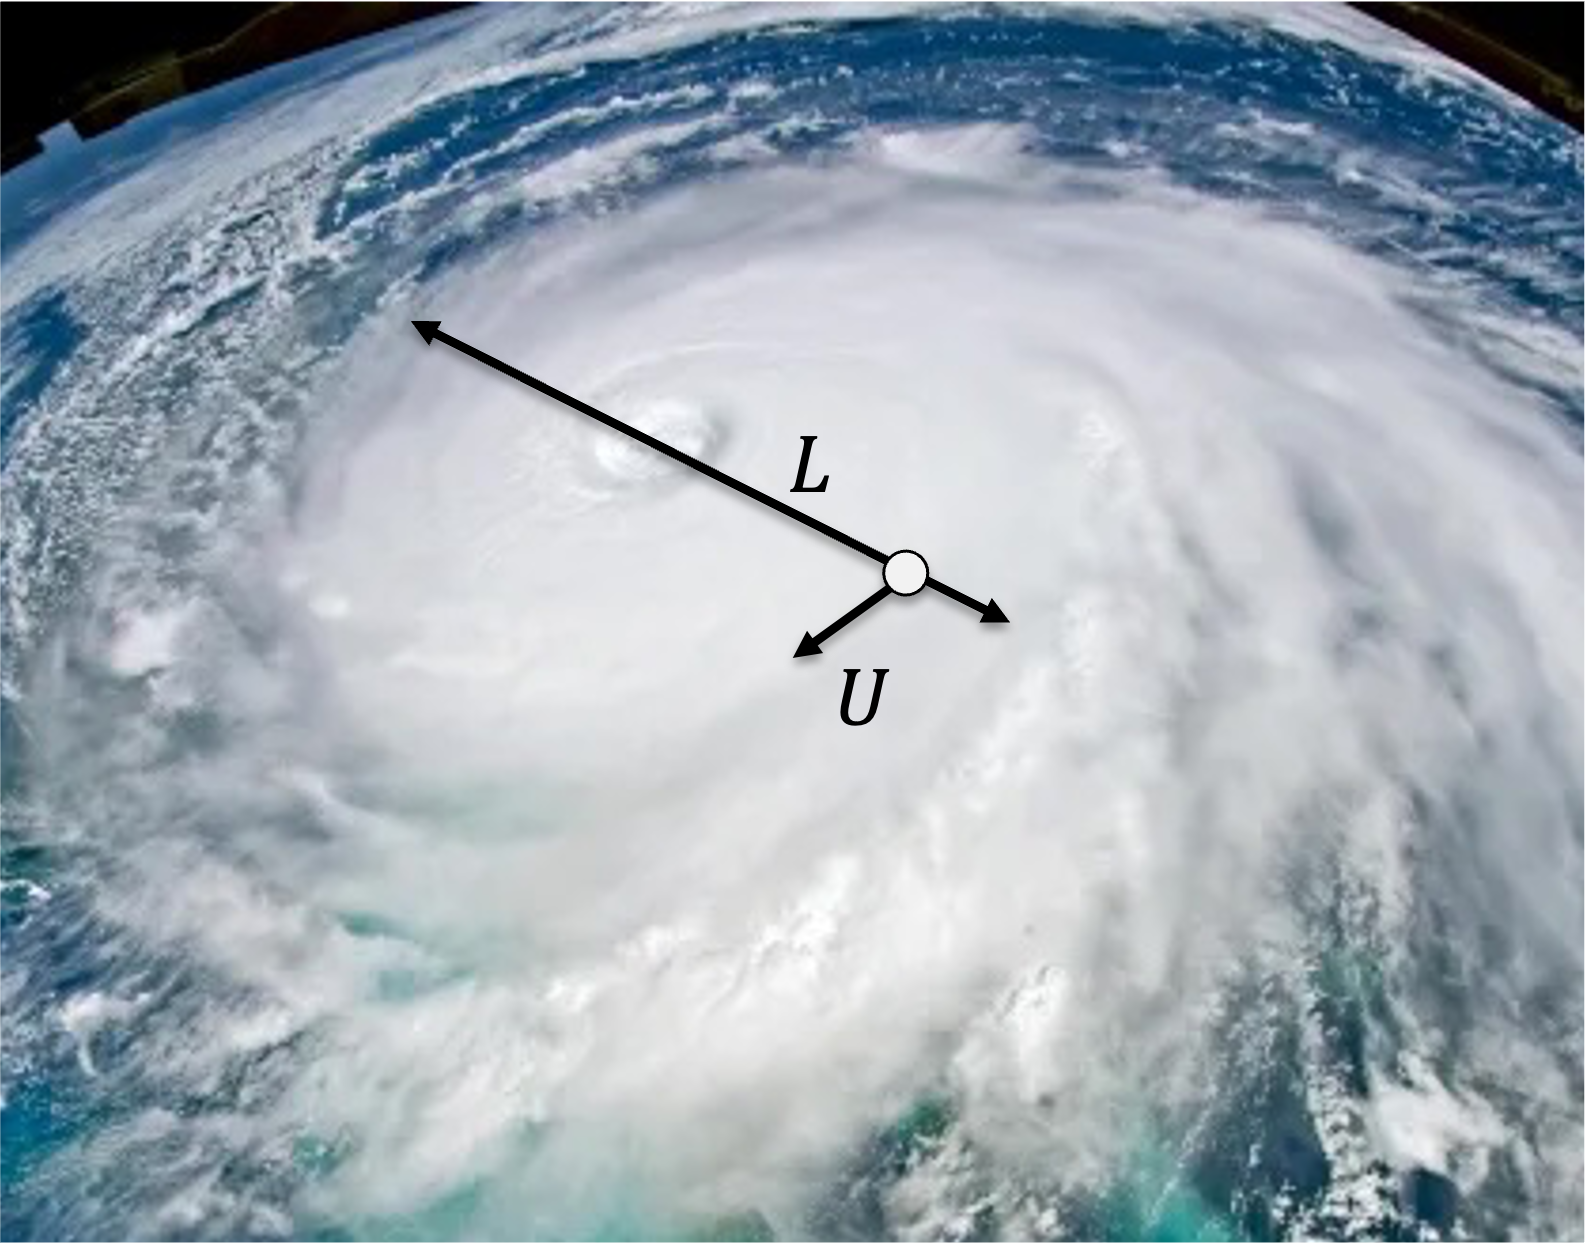
\includegraphics[width=\textwidth]{figs/Fig-nasa-dorian-scale.png}
        \credit{NASA - Hurricane Dorian}{-5pt}
    \end{column}
    \begin{column}{0.4\textwidth}
        The \textbf{length scale} is the diameter of the storm. The \textbf{horizontal velocity scale} is the typical velocity of the flow. And the \textbf{time scale} is approximately the time required for a fluid parcel to move around the storm.
    \end{column}
    
\end{columns}
\end{frame}

\begin{frame}[t]{Atmospheric and ocean dynamics}
\center

\vspace{-1.0em}

\textbf{{\large
Additional strategies
}}

\small 

\vspace{2.0em}

\begin{itemize}
    \item Shallow-water approximation -- assume horizontal length scale is much larger than vertical, integrate over vertical dimension.
    \item Operator splitting, e.g. separation into \emph{geostrophic} and \emph{ageostrophic} components -- longer timesteps possible for slowly evolving terms, reduced computational needs.
    \newline
    \item \textbf{Atmosphere}: Use pressure as the vertical coordinate -- eliminates explicit density dependence, simplifying the continuity equation, and aligns better with the hydrostatic structure of the atmosphere.
    \item \textbf{Ocean}: Rigid lid approximation -- impose a fixed ocean surface, ignores gravitational waves.
\end{itemize}
\end{frame}

% SET THESE FRAMES WITH DIFFERENT BACKGROUND
{\setbeamercolor{background canvas}{bg=mylightgray}

\begin{frame}{Hydrostatic approximation}

Although the horizontal atmosphere is in a
constant state of motion, vertical velocities
are typically fairly small (especially averaged
over the large scale).
\vspace{2em}
\begin{definition}
    A fluid is in \textbf{Hydrostatic balance} when external forces (here gravity) are balanced by the pressure-gradient force, and thus vertical acceleration is zero.
\end{definition}
\vspace{2em}
The \textbf{hydrostatic approximation} assumes that the pressure at any level depends on the weight of the fluid above that level.

%When vertical velocity is approximately zero, density and pressure end up being functionally related.

% Describe hydrostatic approximation

\end{frame}

\begin{frame}{Hydrostatic approximation}

\begin{columns}
\begin{column}{0.5\textwidth}
Forces acting on a given column of air with no vertical acceleration:
   \begin{align*}
       F_\mathrm{T} & =  -\left(p + \delta p \right)\delta A \\
       F_\mathrm{B} & =  p\delta A \\
       F_\mathrm{g} & = -g M = -\rho g \delta A \delta z
   \end{align*}
   A balance of these forces leads to:
   \begin{align*}
       F_T + F_B + F_g = \delta p + \rho g\delta z = 0
   \end{align*}
\end{column}
\begin{column}{0.5\textwidth}
    \begin{center}
    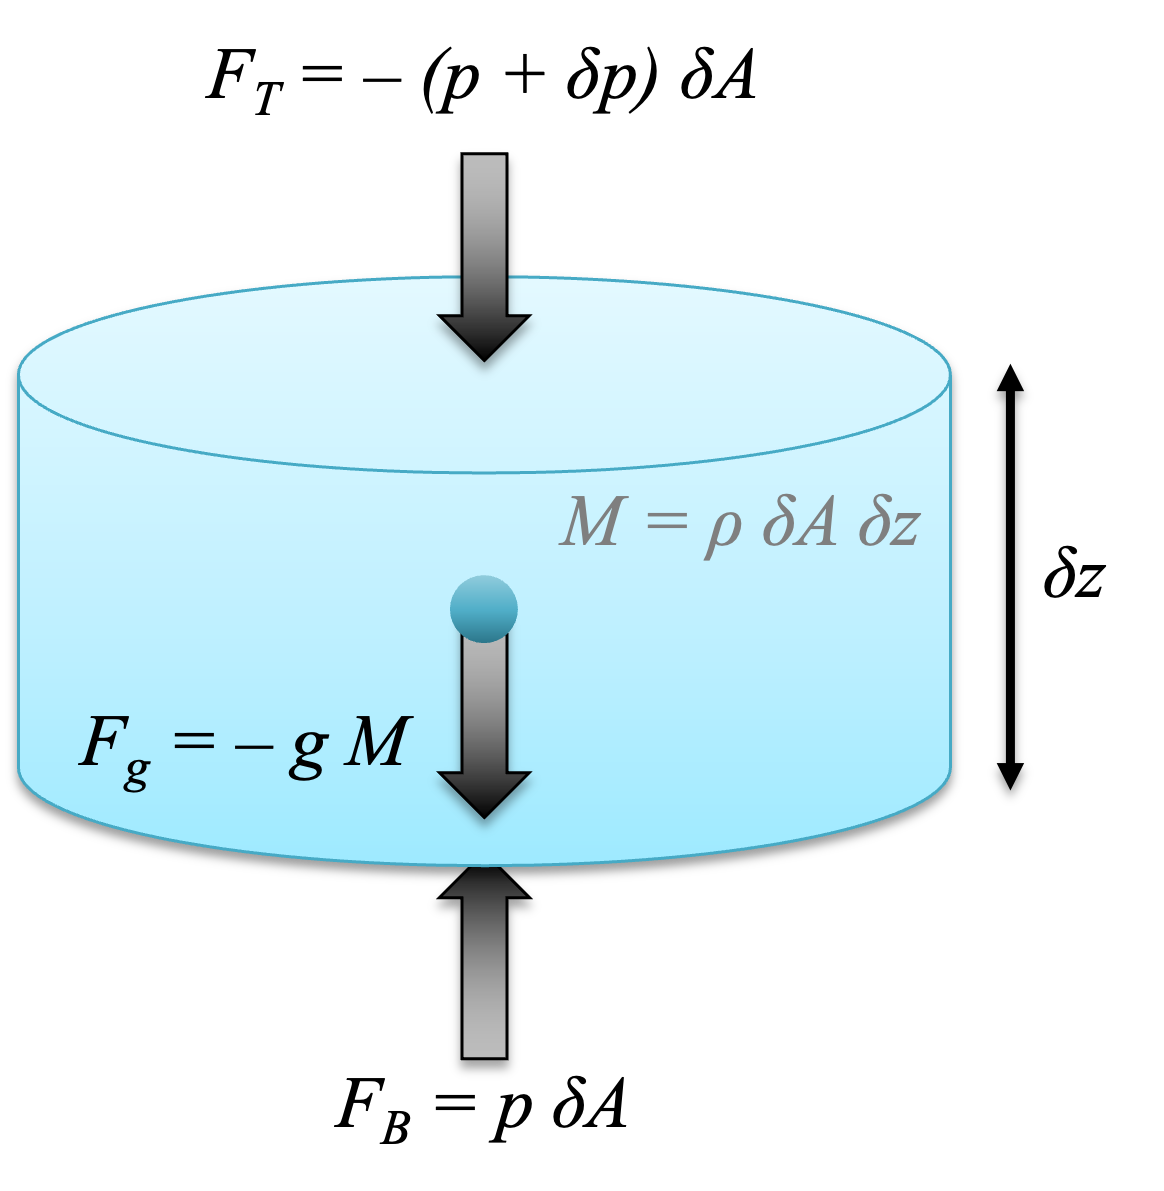
\includegraphics[width=0.7\textwidth]{figs/Fig-Pressure-on-cylinder-ajr.png}
     \end{center}
\end{column}
\end{columns}

\end{frame}

\begin{frame}{Hydrostatic approximation}

\begin{columns}
\begin{column}{0.5\textwidth}
   \begin{align*}
       F_T + F_B + F_g = \delta p + \rho g\delta z = 0
   \end{align*}
   \begin{align*}
       \text{Taylor Series: }\delta p \approx \frac{\partial p}{\partial z}\delta z
   \end{align*}

   Hydrostatic balance:
   \begin{align*}
       \Aboxed{\frac{\partial p}{\partial z} + \rho g = 0}
   \end{align*}
    
\end{column}
\begin{column}{0.5\textwidth}
    \begin{center}
     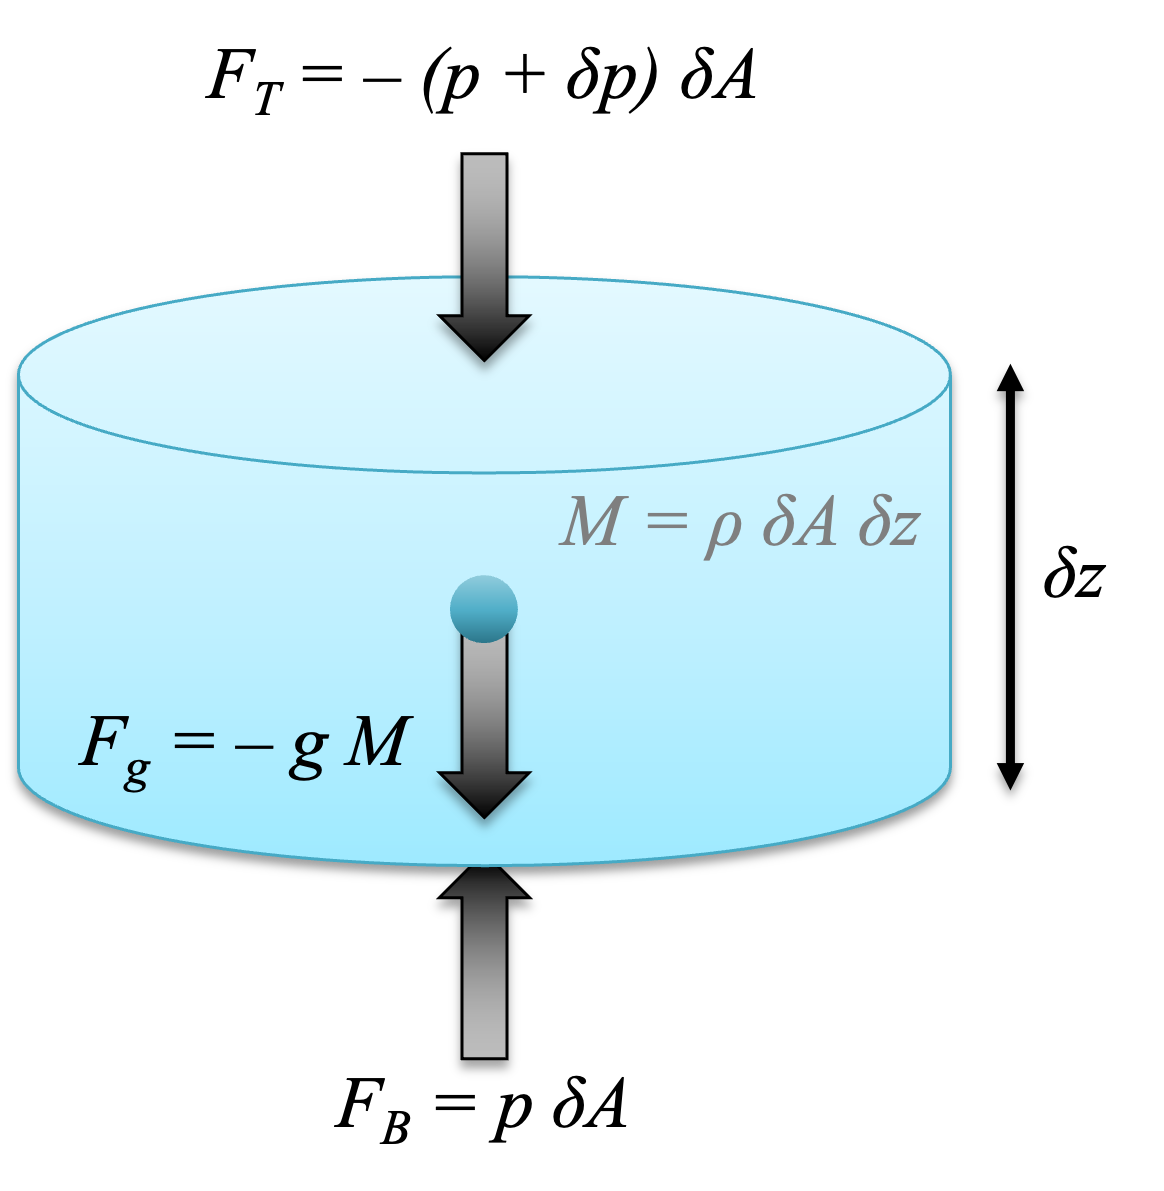
\includegraphics[width=0.7\textwidth]{figs/Fig-Pressure-on-cylinder-ajr.png}
     \end{center}
\end{column}
\end{columns}

\end{frame}

\begin{frame}{Hydrostatic approximation}

\begin{columns}
\begin{column}{0.5\textwidth}
   \begin{align*}
       F_T + F_B + F_g = \delta p + \rho g\delta z = 0
   \end{align*}
   \begin{align*}
       \text{Taylor Series: }\delta p \approx \frac{\partial p}{\partial z}\delta z
   \end{align*}

   Hydrostatic balance:
   \begin{align*}
       \Aboxed{\frac{\partial p}{\partial z} + \rho g = 0}
   \end{align*}
    
\end{column}
\begin{column}{0.5\textwidth}
    Integrating from the top of the atmosphere downward, and noting that $p(z=\infty)=0$ then gives the pressure at any level $z$:
    \begin{align*}
        p(z) = g \int_z^\infty \rho dz
    \end{align*}
\end{column}
\end{columns}

\end{frame}

} % END FRAME COLOR %%%%

\begin{frame}[t]{Atmospheric and ocean dynamics}

\vspace{-1.0em}

\begin{columns}
    \begin{column}[t]{0.6\textwidth}
        \begin{center}
        \textbf{{\large
        Non-hydrostatic conditions
        }}
        \end{center}
        
        \vspace{1.5em}
        
        When does the hydrostatic approximation fail?
        \\[1em]
        $\Longrightarrow$ When vertical velocity is not small, like for localized convection and near steep topography. 
        \newline
        \newline
        If these cases are of interest, then it is important to consider the full \textbf{non-hydrostatic} equations.
    \end{column}
    \begin{column}[t]{0.4\textwidth}
        \centering
        
        % figure from:
        %https://brian-rose.github.io/ClimateLaboratoryBook/courseware/climate-system-models.html
        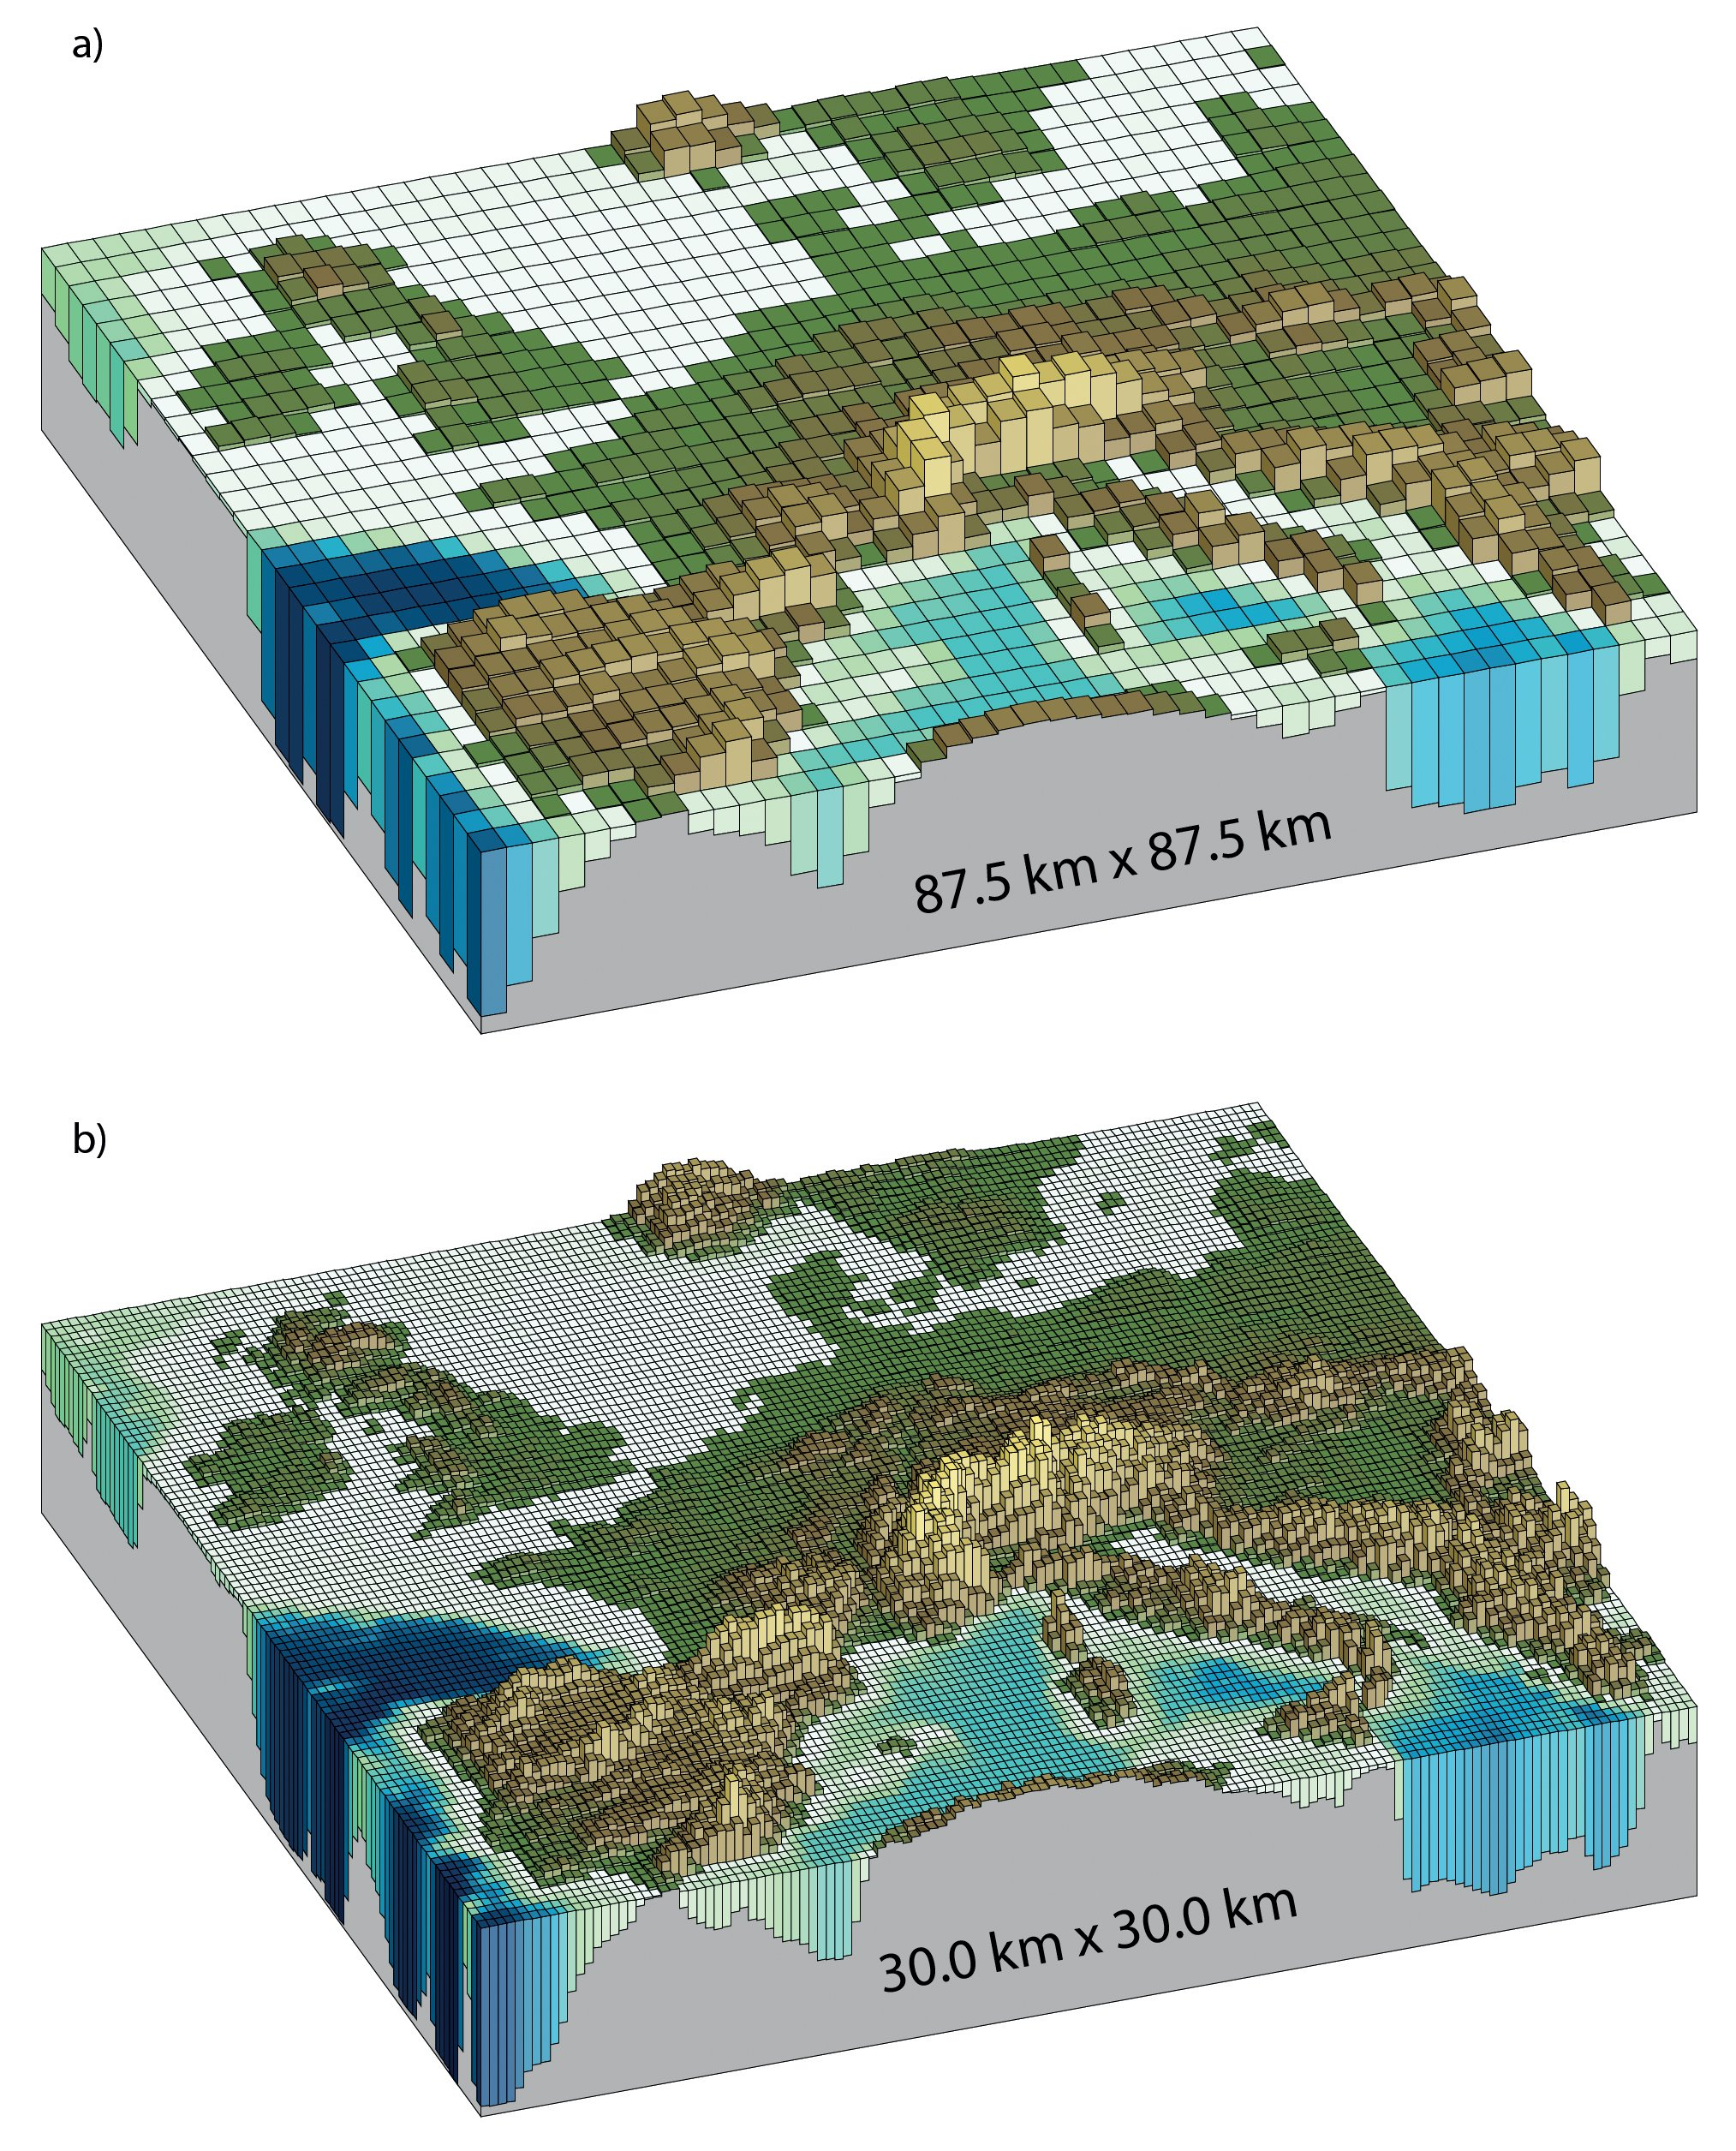
\includegraphics[width=0.9\textwidth]{figs/Fig-gcm-resolution-Fig1-14.jpg}
        \credit{Rose, 2020}{5pt}
    \end{column}
\end{columns}
        
\end{frame}

\begin{frame}[t]{Ice-sheet dynamics}

\vspace{-1.0em}

\begin{center}
\textbf{{\large
Flow regimes
}}
\end{center}

\footnotesize 
\centering

\vspace{-0.5em}

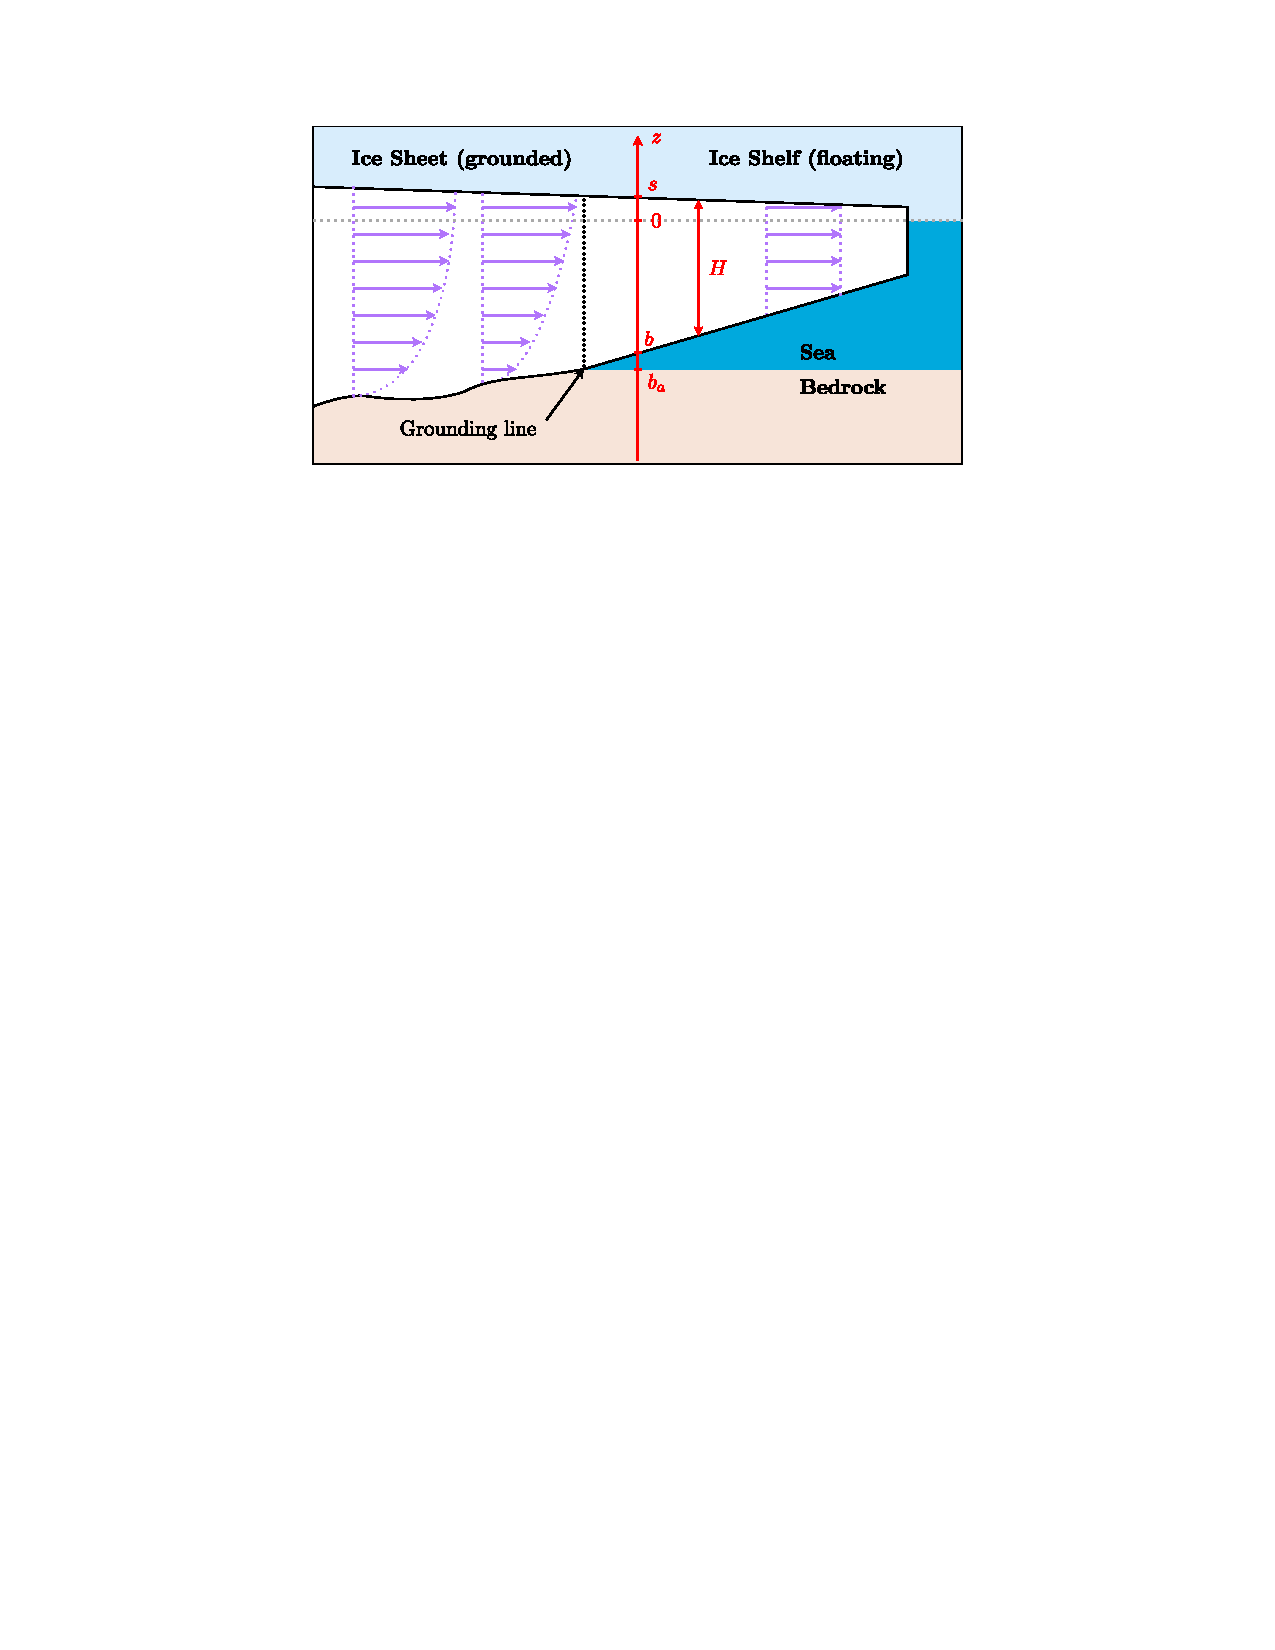
\includegraphics[width=0.75\textwidth]{figs/Fig-ice-flow-regimes-larour2012.pdf}
\credit{Larour et al., 2012}{50pt}

\end{frame}

\end{document}